%%%%%%%%%%%%%%%%%%%%%%%%%%%%%%%%%%%%%%%%%
% Based on template downloaded from:
% http://www.LaTeXTemplates.com
%
% Original author:
% Linux and Unix Users Group at Virginia Tech Wiki 
% (https://vtluug.org/wiki/Example_LaTeX_chem_lab_report)
%
% License:
% CC BY-NC-SA 3.0 (http://creativecommons.org/licenses/by-nc-sa/3.0/)
%
%%%%%%%%%%%%%%%%%%%%%%%%%%%%%%%%%%%%%%%%%
\documentclass{article}

\usepackage[version=3]{mhchem} % Package for chemical equation typesetting
\usepackage{siunitx} % Provides the \SI{}{} and \si{} command for typesetting SI units
\usepackage{graphicx} % Required for the inclusion of images
\usepackage{natbib} % Required to change bibliography style to APA
\usepackage{amsmath} % Required for some math elements 
\usepackage{listings}
\usepackage{xcolor}


\definecolor{codegreen}{rgb}{0,0.6,0}
\definecolor{codegray}{rgb}{0.5,0.5,0.5}
\definecolor{codepurple}{rgb}{0.58,0,0.82}
\definecolor{backcolour}{rgb}{0.95,0.95,0.92}

\lstdefinestyle{mystyle}{
    backgroundcolor=\color{backcolour},   
    commentstyle=\color{codegreen},
    keywordstyle=\color{magenta},
    numberstyle=\tiny\color{codegray},
    stringstyle=\color{codepurple},
    basicstyle=\ttfamily\footnotesize,
    breakatwhitespace=false,         
    breaklines=true,                 
    captionpos=b,                    
    keepspaces=true,                 
    numbers=left,                    
    numbersep=5pt,                  
    showspaces=false,                
    showstringspaces=false,
    showtabs=false,                  
    tabsize=2
}

\lstset{style=mystyle}

\setlength\parindent{0pt} % Removes all indentation from paragraphs

\renewcommand{\labelenumi}{\alph{enumi}.} % Make numbering in the enumerate environment by letter rather than number (e.g. section 6)

%\usepackage{times} % Uncomment to use the Times New Roman font

%----------------------------------------------------------------------------------------
%	DOCUMENT INFORMATION
%----------------------------------------------------------------------------------------

\title{\textbf{REMODEL automated report} \\ A Community Poll on Reproducibility in Computational Geosciences} % Title

\author{Robert \textsc{Reinecke}} % Author name

\begin{document}

\maketitle % Insert the title, author and date

\begin{center}
\begin{tabular}{l r}
Report last updated: & May 27, 2021\\
Compilation date: & \today
\end{tabular}
\end{center}

This document summerizes a full analysis for detailed results. \textbf{It is not a full publication but rather an automated representation of the data present in this repository.}

It summarizes the extensive results and builds the foundation for the publication of a journal paper.
It will also be distributed along with the data in the course of a journal and data publication.

\thispagestyle{empty}

\tableofcontents
\listoffigures

\newpage

\section{Aim of this survey}
Software development has become an integral part of the geosciences$^{1}$ as models and data processing get more sophisticated.
Paradoxically, it poses a threat to scientific progress as the pillar of science, reproducibility, is seldomly reached$^{2}$.
Software code tends to be either poorly written and documented or not shared at all; proper software licenses are rarely attributed.
This is especially worrisome as scientific results have potential controversial implications for stakeholders and policymakers and may influence the public opinion for a long time$^{3}$.

In recent years, progress towards open science has led to more publishers demanding access to data and source code alongside peer-reviewed manuscripts4,5. Still, recent studies find that results can rarely be reproduced $^{6,7}$.

In this project, we conduct a poll among the geoscience community which is advertised via scientific blogs (AGU, EGU), research networks (researchgate.net and mailing lists), and social media.
Therein, we strive to investigate the causes for that lack of reproducibility.
We take a peek behind the curtain and unveil how the community develops and maintains complex code and what that entails for reproducibility$^{8}$ .
Our survey includes background knowledge, community opinion, and behaviour practices regarding reproducible software development.

We postulate that this lack of reproducibility$^{9}$  might be rooted in insufficient reward within the scientific community, insecurity regarding proper licencing of software and other parts of the research compendium as well as scientists’ unawareness about how to make software available in a way that allows for proper attribution of their work.
We question putative causes such as unclear guidelines of research institutions or that software has been developed over decades$^{10}$ , by researchers' cohorts without a proper software engineering process¹ and transparent licensing.

To this end, we also summarize solutions like the adaption of modern project management methods from the computer engineering community$^{11}$  that will eventually reduce costs while increasing the reproducibility of scientific research$^{8}$ .

1 A comment to "Most Computational Hydrology is not Reproducible, so is it Really Science?” R.W. Hut, N.C. van de Giesen, N. Drost, Water Resources Research, 2017\\
2 Hutton, C., Wagener, T., Freer, J., Han, D., Du\_y, C., and Arheimer, B., Most computational hydrology is not reproducible, so is it really science? Water Resources Research, 2016\\
3 Munafò, M., Nosek, B., Bishop, D. et al., A manifesto for reproducible science. Nat Hum Behav, 2017\\
4 Executive editors, G. Editorial: The publication of geoscientifc model developments v1.2. Geoscientifc Model Development, 2019\\
5 Katz, D. S., Niemeyer, K. E., and Smith, A. M., Publish your software: Introducing the journal of open source software (joss), Computing in Science Engineering, 2018\\
6 Stagge, J. H., Rosenberg, D. E., Abdallah, A. M., Akbar, H., Attallah, N. A., and James, R., Assessing data availability and research reproducibility in hydrology and water resources. Scientific data, 2019\\
7 Añel, J. A., García-Rodríguez, M., and Rodeiro, J.: Current status on the need for improved accessibility to climate models code, Geosci. Model Dev., 2021\\
8 Stodden, V., The reproducible research standard: Reducing legal barriers to scientific knowledge and innovation. IEEE Computing in Science \& Engineering, 2009\\
9 https://www.nature.com/news/1-500-scientists-lift-the-lid-on-reproducibility-1.19970\\
10 Muller, C., Schaphoff, S., von Bloh, W., Thonicke, K., and Gerten, D., Going open-source with a model dinosaur and establishing model evaluation standards. EGU, 2018\\
11 https://software.rajivprab.com/2019/11/25/the-birth-of-legacy-software-how-change-aversion-feeds-on-itself\\


Our larger questions:
\begin{itemize}
	\item Is eproducibility is an issue in the geosciences? Are bad code and documentation the root cause of that issue?
	\item Is model software too complex? Does that hinder reproducibility?
	\item Are researchers missing the tools and know-how (methods, licenses etc.) to build good model code?
	\item Is missing funding and missing time preventing researchers from making their models more accessible?
\end{itemize}

We define reproducibility as:

"Reproducibility in the context of modeling in the geosciences means that results obtained by a modeling experiment should be achieved again with a high degree of agreement when the study is replicated with the same model design, inputs, and general methodology by different researchers.

We explicitly exclude the retracing of results by means of using a different modeling environment (including variations in model concept, algorithms, input data or methodology)."

\section{Data processing}
We designed the survey according to standards from psychology research. We apply descriptive statistics to analyse demographic background and basic analysis.
Further, we apply inferential statistical methods to test the unerlying hypotheses.

The raw data of the survey is stored in the folder \textbf{LiveData}. \textbf{The raw data has not been modified or cleaned in any way.}
To run some basic cleanup run the follwoing script: 

\begin{lstlisting}[language=Python]
import process_data.py as p
p.process()
\end{lstlisting}

\section{Results}
All data processing and plotting (including building this document) can be executed by running \lstinline{python run.py}.
Plotting details and addtional processing can be found in th script \lstinline{plot_all.py}.

Our main hypothesis for this analysis where the following:
\begin{itemize}
	\item \textbf{H1} Young scientists develop software more actively than established researchers.
	\item \textbf{H2} Young scientists are more familiar with software licenses than established researchers. 
	\item \textbf{H3} Young scientists are more familiar with modern development methods than established researchers. 
	\item \textbf{H4} Senior researcher percieve reproducability as a lesser problem than early career researchers.
 	\item \textbf{H5} Software complexity is the main reason for a lack of reproducability.
 	\item \textbf{H6} Researchers code frequently but without knowledge about proper engineering methods, licences and tools. 
 	\item \textbf{H7} The most frequently used language is still C/Fortran. Younger scientists tend to use Python and R; this is consistent throughout fields 
 	\item \textbf{H8} Most researchers are autodidacts when it comes to coding. 
 	\item \textbf{H9} Most researchers have never reproduced code with the original model. Only with their own model. This differs between fields. 
 	\item \textbf{H10} Practitioners and researchers perceive the issue of reproducibility differently. Scientists are more aware (?). 
	\item \textbf{H11} There are more researchers that apply software than they are ones that develop it. This differs between activities and fields. 
 	\item \textbf{H12} Most researcher do not know if their software belongs to them. 
 	\item \textbf{H13} Models that are available are hard to use. Causes?: Bad code, no documentation, no input data 
 	\item \textbf{H14} Senior researchers are convinced their work is reproducible. (much more at least than young scientists) 
 	\item \textbf{H15} The smaller the scale the more reproducible and accessible. 
 	\item \textbf{H16} Researchers think that their software is bug free and always correspond to their intended implementation. 
 	\item \textbf{H17} Most senior scientists think investment in FOSS doesn’t pay off. 
 	\item \textbf{H18} Senior researchers think that their code/project is easier to understand but that conflicts with reality. And younger researchers have the opposite understanding. 
 	\item \textbf{H19} We need more funding to enable reproducible computational science. 
\end{itemize}

\subsection{Sample Characteristics (demographics)}
Who were our participants?
Here we present characteristics of the participants in our poll, i.e. their current career stage, their years of research experience, their geo-scientific field and scale as well as their current focus of work.
This is purely descriptive statistics.
As we welcomed everyone to our poll, we did not form any assumptions regarding sample characteristics.
Also, we tried, but might not have reached a representative sample of the population of geo-scientists.

Here, we report basic sample characteristics. Also, we can check for and report any salient sample properties.

Corresponding survey questions:

\begin{itemize}
	\item DM01 - What career stage are you in?
	\item DM02 - For how long have you been working in your research field?
	\item DM06 - To which field within the geosciences does your research mainly belong?
	\item DM05 - What geographic scale are you working on?
	\item DM07 - What is the focus of your work?
\end{itemize}

\begin{figure}[!p]
    \centering
    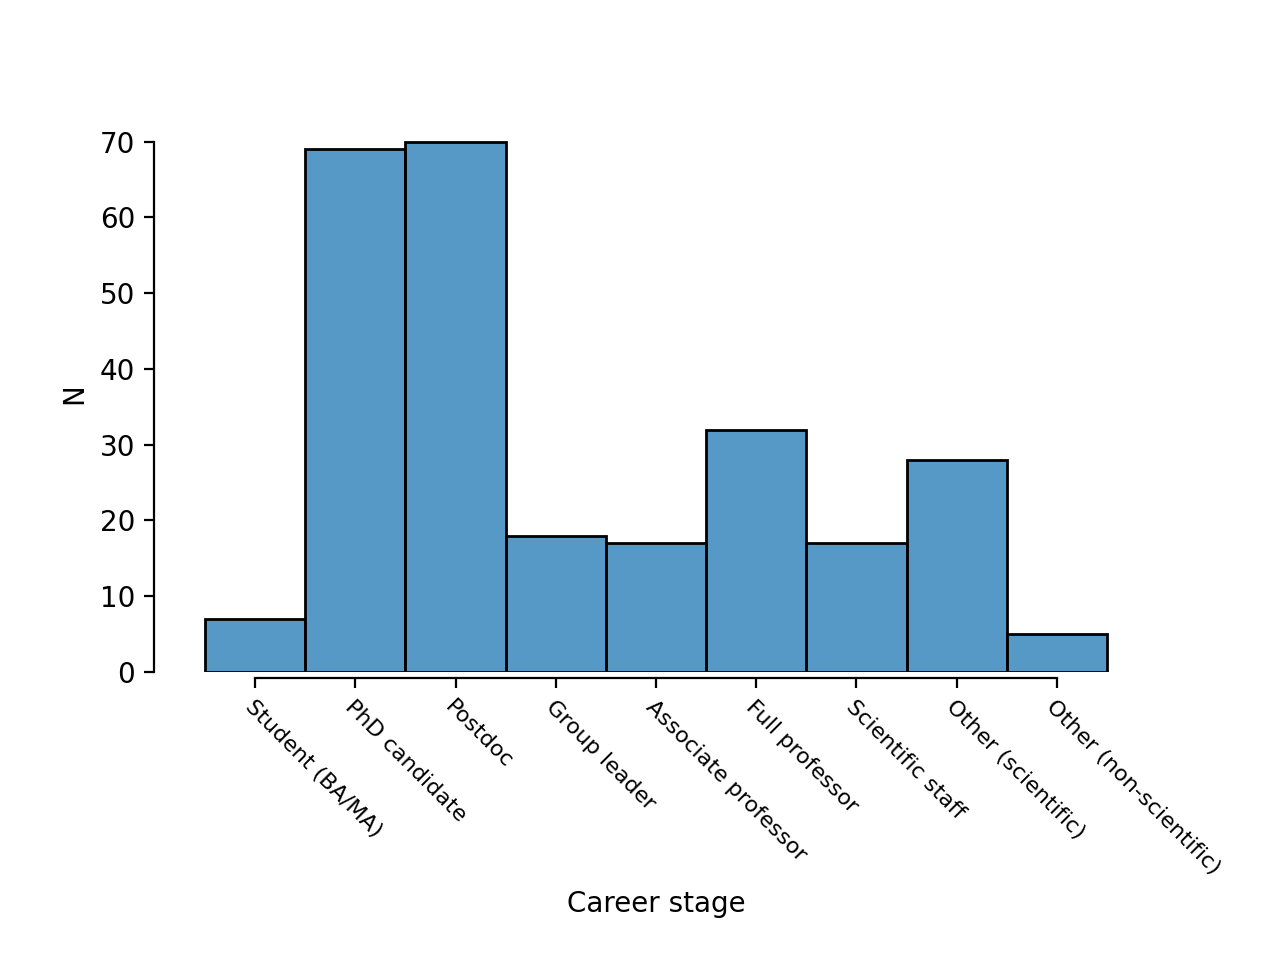
\includegraphics[width=\textwidth]{../figs/DM01.png}
	\caption{DM01 - Career stage of participants}
    \label{fig:dm01}
\end{figure}

\begin{figure}[!p]
    \centering
    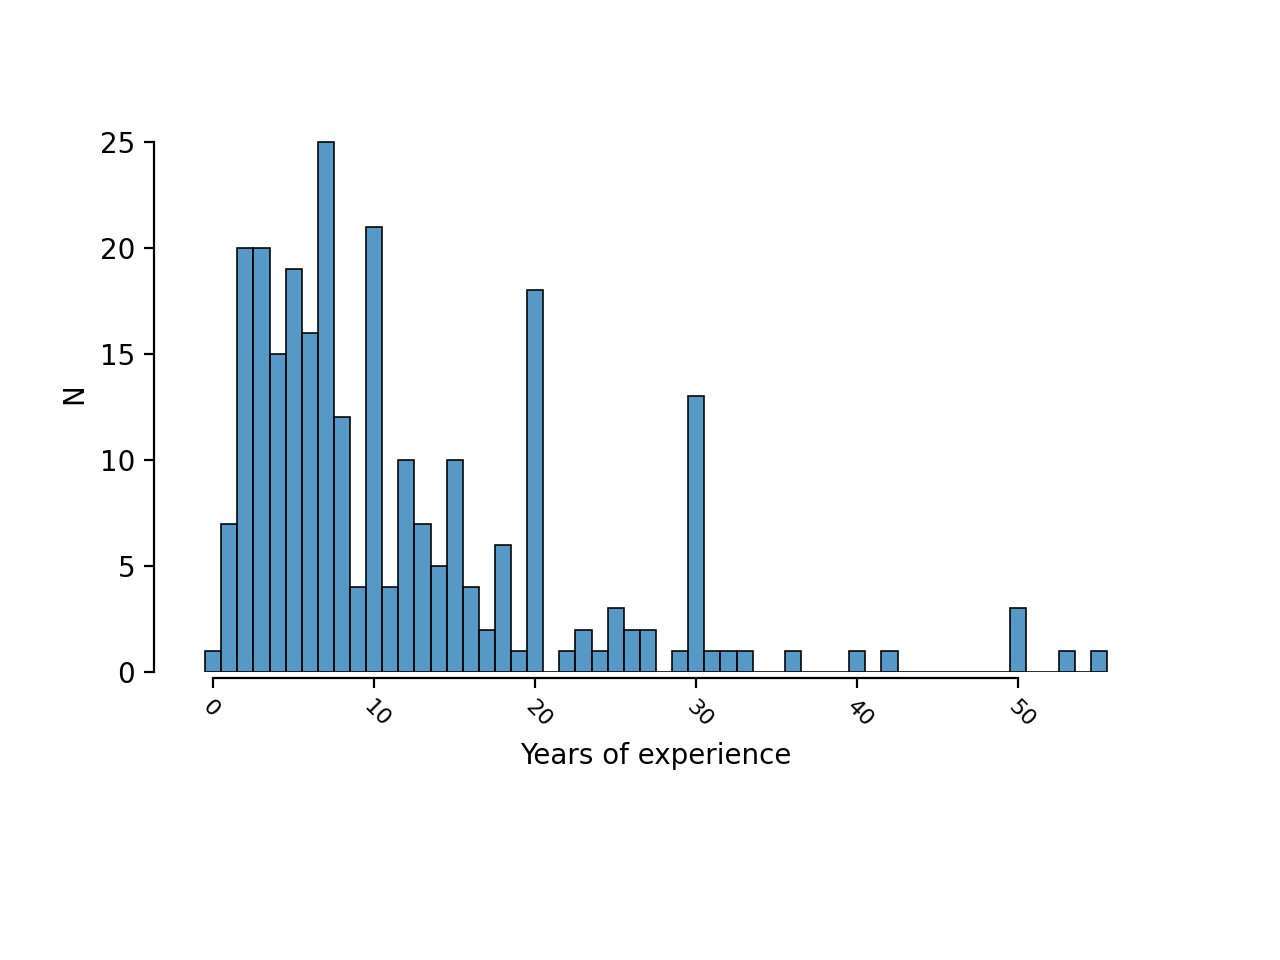
\includegraphics[width=\textwidth]{../figs/DM02_01.png}
	\caption{DM02 - For how long have you been working in your field?}
    \label{fig:dm02}
\end{figure}

\begin{figure}[!p]
    \centering
    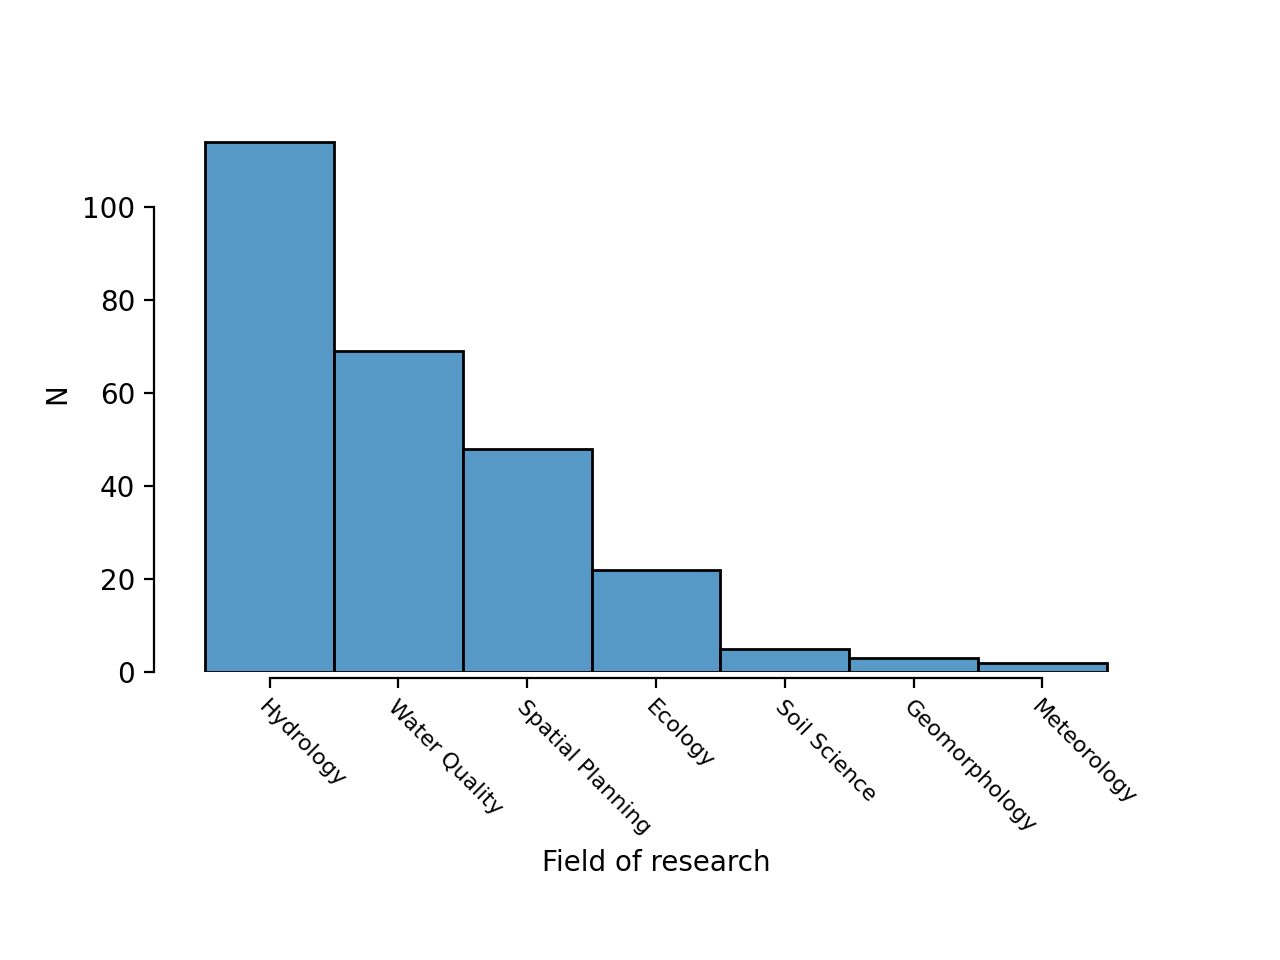
\includegraphics[width=\textwidth]{../figs/DM06.png}
	\caption{DM06 - Which field do you belong to?}
    \label{fig:dm06}
\end{figure}

\begin{figure}[!p]
    \centering
    \includegraphics[width=\textwidth]{../figs/DM05.png}
	\caption{DM05 - What scale are you working on?}
    \label{fig:dm05}
\end{figure}

\begin{figure}[!p]
    \centering
    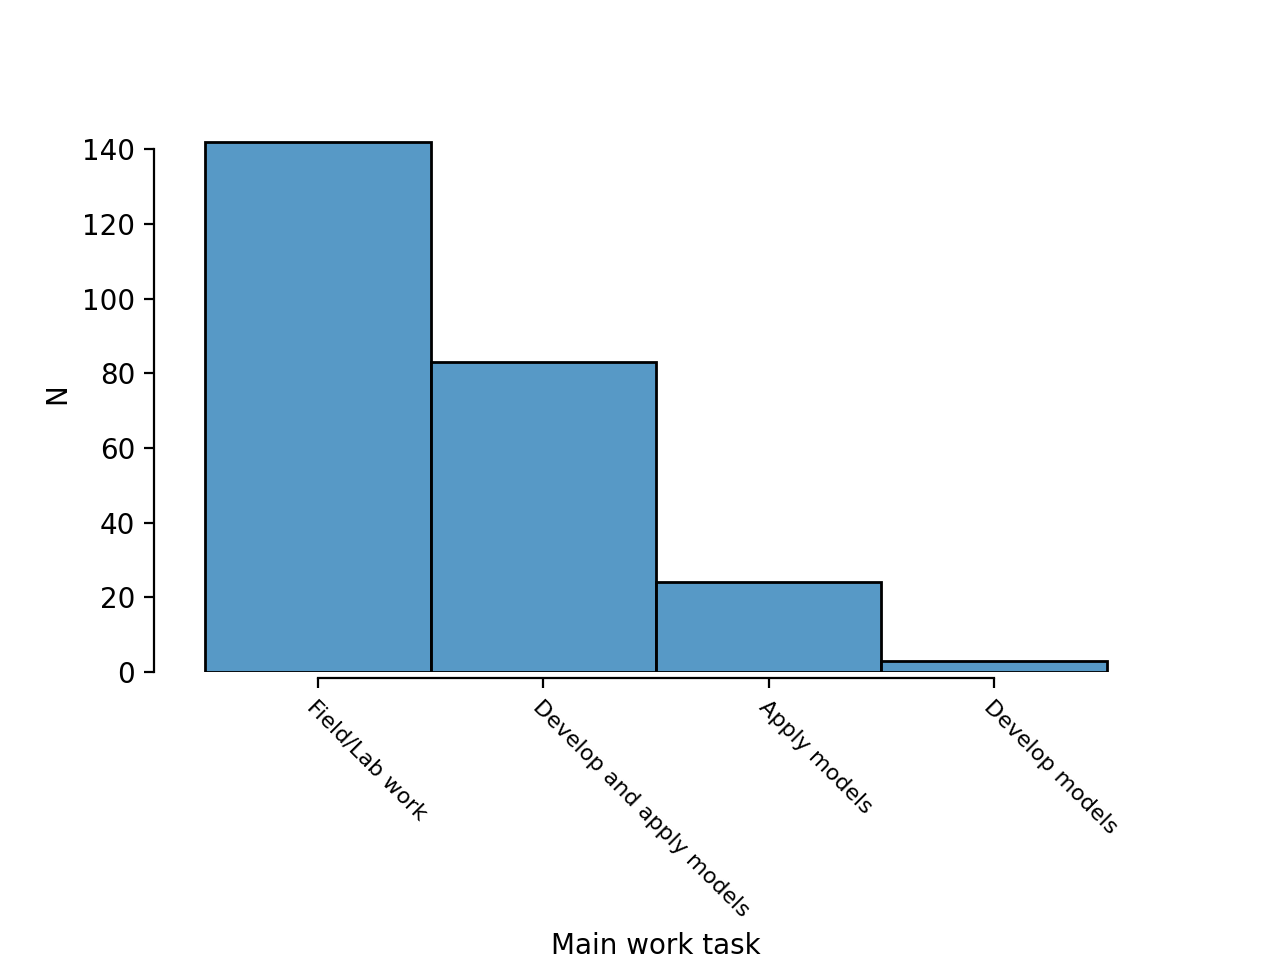
\includegraphics[width=\textwidth]{../figs/DM07.png}
	\caption{DM07 What is the focus of your work?}
    \label{fig:dm07}
\end{figure}
\newpage

\subsection{Community Opinion on Reproducibility}
This part covers people's view and opinion. We assume that our defintion of reproducibility was used (annotated at several points in the poll).

This part focuses on how reproducibility is perceived by different researchers and what the causes are for limited reproducibility.

We expected that early career scientists are more aware of the problem than senior scientists. We further expected that a main cause for a lack of reproducibility is the lack of accessible code and input data.

Corresponding survey questions:
\begin{itemize}
	\item O101 - How strongly do you agree with the following statements?
	\item O103 - What are the reasons for a lack of reproducibility?
	\item S113 - How long do you think does it take for an average PhD student to efficiently work with your research software?
\end{itemize}

Corresponding hypotheses
\begin{itemize}
	\item H4 Senior researcher percieve reproducability as a lesser problem than early career researchers.
 	\item H5 Software complexity is the main reason for a lack of reproducability.
	\item H10 Practitioners and researchers perceive the issue of reproducibility differently. Scientists are more aware (?).
	\item H13 Models that are available are hard to use. Causes?: Bad code, no documentation, no input data.
	\item H14 Senior researchers are convinced their work is reproducible. (much more at least than young scientists).
	\item H16 Researchers think that their software is bug free and always correspond to their intended implementation.
\end{itemize}

O101: Opinion on Reproducibility in Geo-Sciences: How strongly did participants generally agree with statements?
Do they consider it a problem at all? Do they think that their work is reproducible?

\begin{figure}[!p]
    \centering
    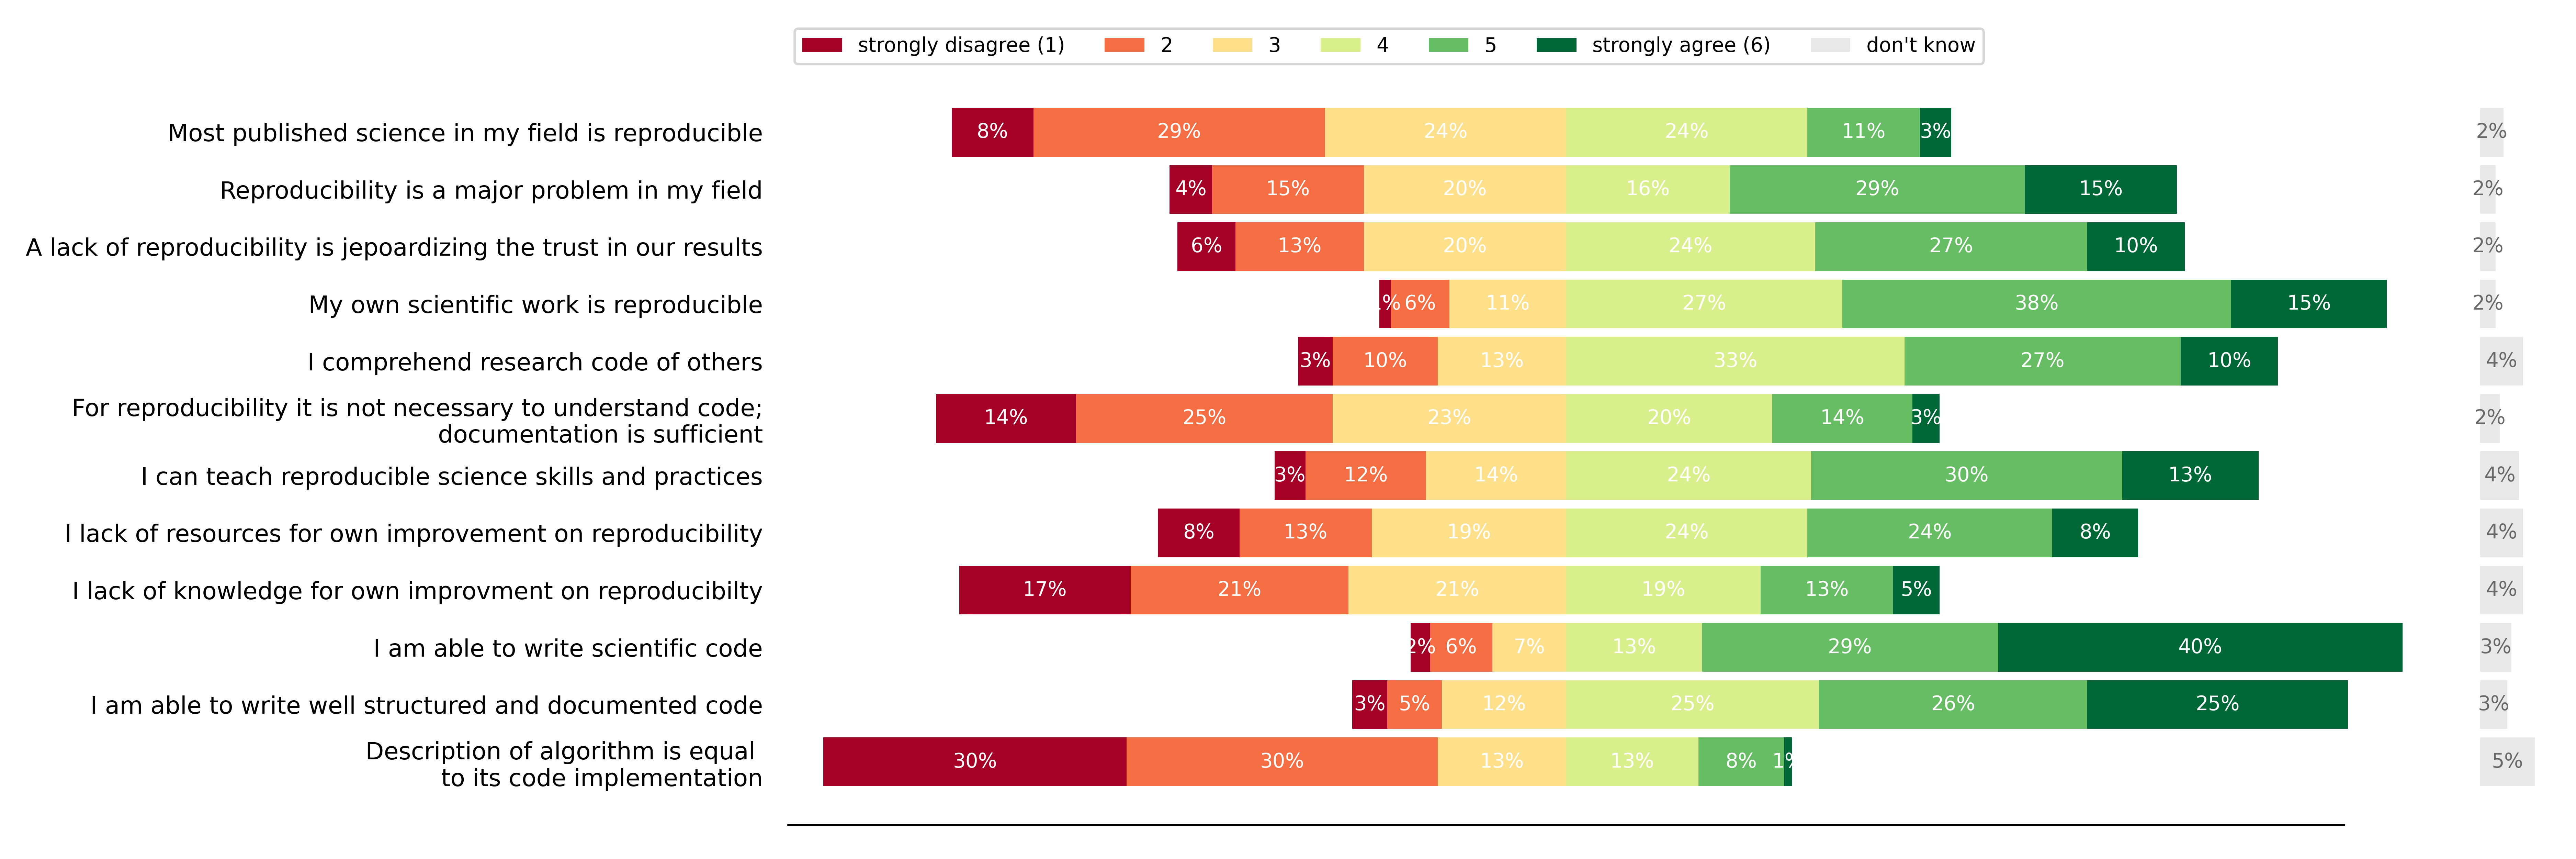
\includegraphics[width=\textwidth]{../figs/O101.png}
	\caption{O101 How strongly do you agree with the following questions?}
    \label{fig:O101}
\end{figure}

\begin{figure}[!p]
    \centering
    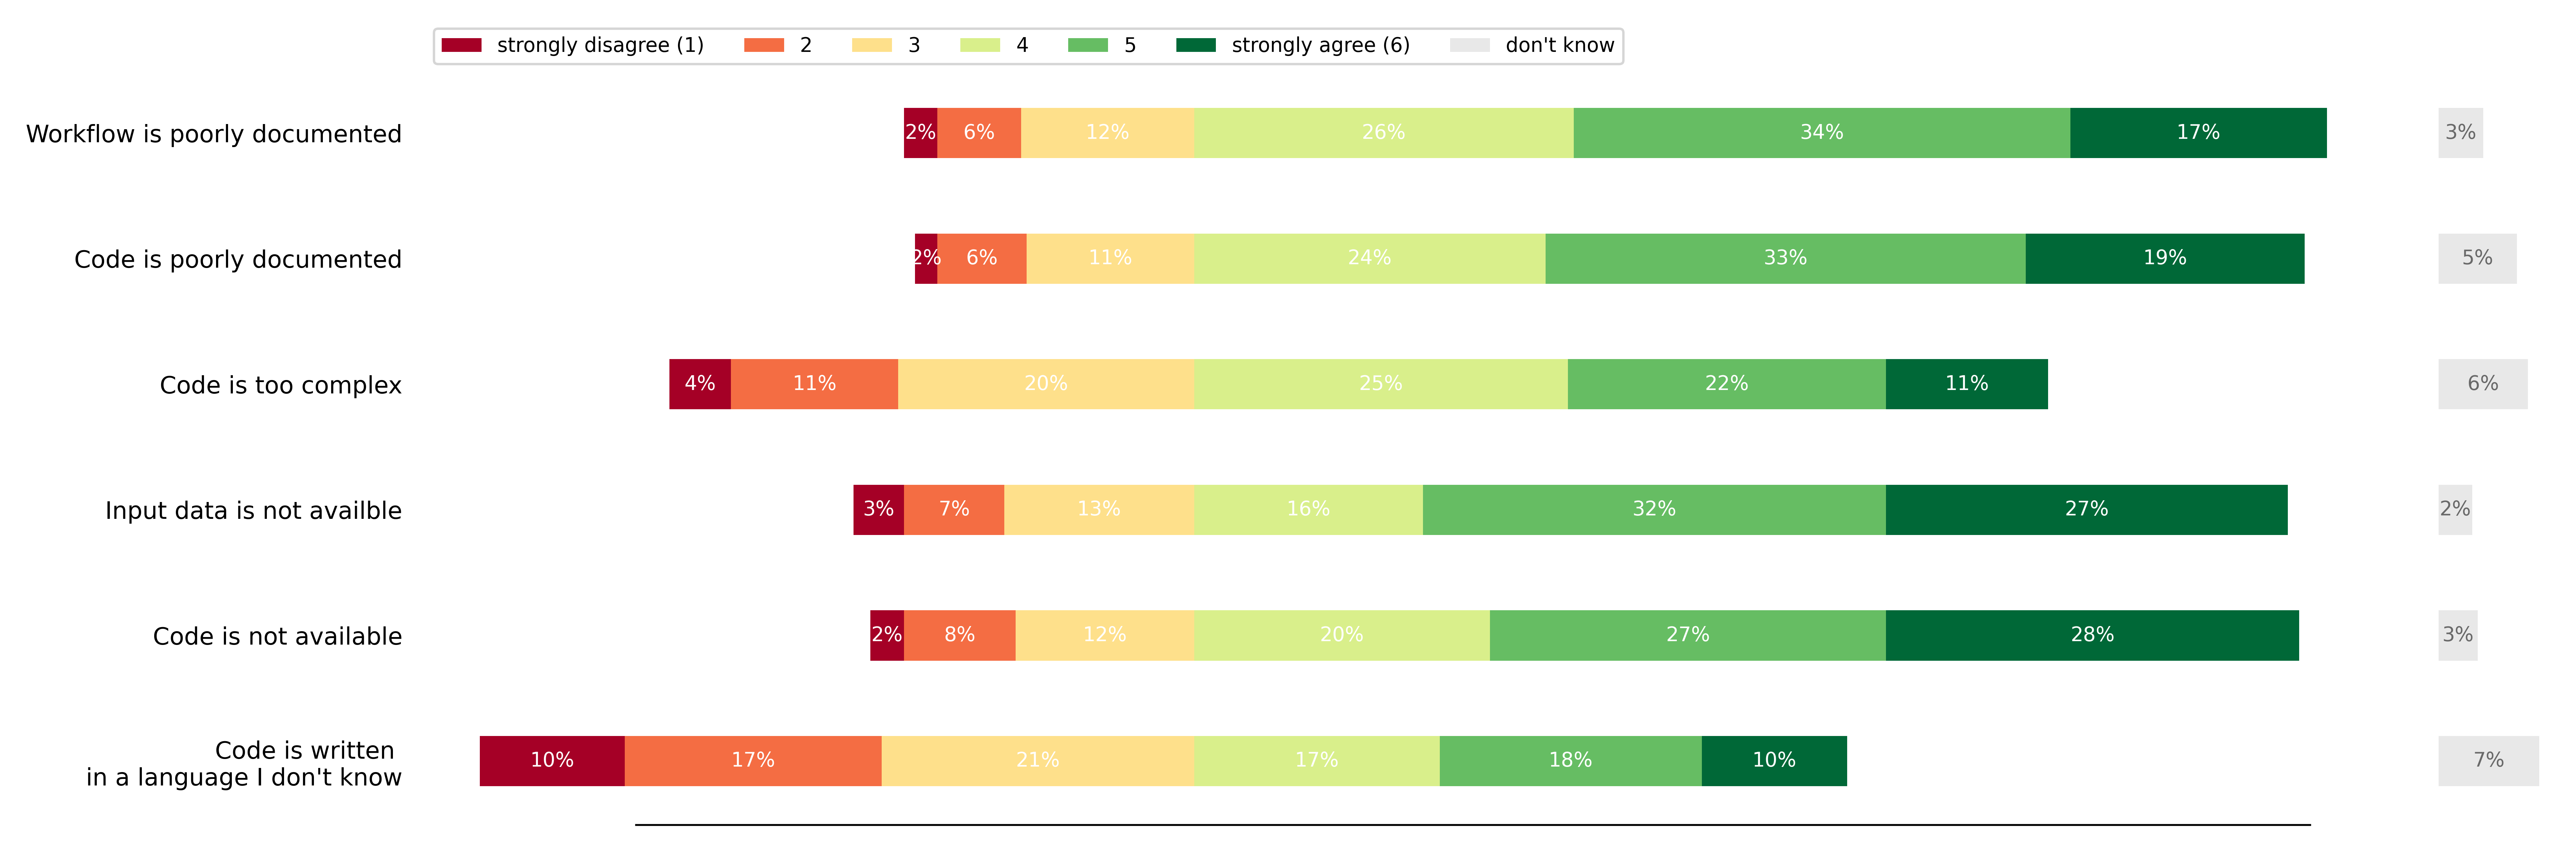
\includegraphics[width=\textwidth]{../figs/O103.png}
	\caption{O103 What are the reasons for poor reproducibility?}
    \label{fig:O103}
\end{figure}

\begin{figure}[!p]
    \centering
    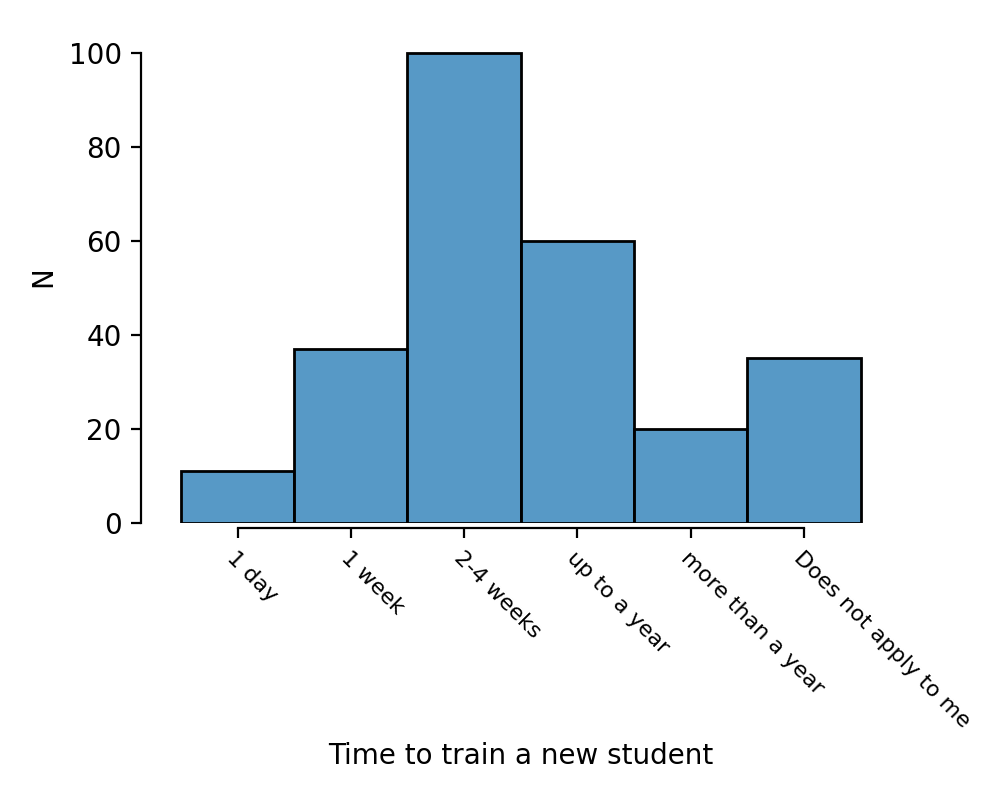
\includegraphics[width=\textwidth]{../figs/S113.png}
	\caption{S113 How long does it take to train a new student in your software?}
    \label{fig:S113}
\end{figure}

\newpage

\subsubsection{H4 Differences in Opinion on Reproducibility}

Number of established (full Prof.) researchers: 32

Number of young (Students, PhD candidates, Postdocs, Junior Prof., Associate Prof.) researchers: 181

Mean agreement to reproducibility: 3.105058

Mean agreement among young sc.: 3.005650

Mean agreement among established sc.: 3.612903

Median agreement to reproducibility: 3.000000

Median agreement among young sc.: 3.000000

Median agreement among established sc.: 4.000000
Career has no normal distribution

No statistical test possible, samples of to low to do a proper Wilcoxon or even t-test


\subsubsection{H5 Reasons for lack of reproducibility}


All answers (without don't know) -  Mean workflow: 4.390438, code documentation : 4.440816, code complexity: 3.884774, input data not available: 4.501976, code availability: 4.500000, written language: 3.473029

Thus, the main reason for a lack of reproducibility is: Input data, then 2: code availability, 3: documentation, 4: workflow, 5: code complexity, 6: language

Mean agreement code complexity 3.884774

Mean agreement among young sc.: 3.784431

Mean agreement among established sc.: 4.033333

Median agreement: 4.000000

Median agreement among young sc.: 4.000000

Median agreement established sc: 4.000000


\subsubsection{H10 Practitioners are less awarte of the issue}

No Data to investiagte this question. Only scientists answered the poll.

\subsubsection{H13 Reasons for reproducibility}

See H5. No addtional data to explore this further.

\subsubsection{H14 Senior researchers are convinced their work is reproducible. (much more at least than young scientists).}


Mean agreement on: my own research is reproducible: 4.428571

Mean agreement among young sc.: 4.413408

Mean agreement among estbalished sc: 4.562500

Median agreement: 5.000000

Median agreement among young sc: 5.000000

Median agreement among established sc.: 5.000000


\subsubsection{H16 Researchers think that their software is bug free and always correspond to their intended implementation.}
We did not ask a question that perfectly relates. Parts are answered in Fig. \ref{fig:O101}.
Main relation to question: Implementing an algorithm based on a description from a publication yourself is the same as using the exact software package/original code that was used in that very publication.


Mean agreement - description is same as implementation: 2.379592


\newpage

\subsection{Reproducibility Practices and Skills}
This part covers "actual" behaviour. This is only a self-report assessment.

Summarized, we wanted to know if researchers actively participate in reproducing results. Furthermore, we were intrested in finding out what kind of tools and licences they use to publish their own results.

We expected to see that that less than 50\% are actively repoducing results and that general knowledge about tools and licenses is low.

Corresponding hypotheses
\begin{itemize}
	\item H6 Researchers code frequently but without knowledge about engeneering methods licences and tools.
	\item H9 Most researchers have never reproduced code with the original model. Only with their own model. This differs between fields.
	\item H12 Most researchers don't know if their software belongs to them.
	\item H2 Young scientists are more familiar with licencing issues.
	\item H7 The most frequently used language is still C/Fortran. Younger scientists tend to use Python and R
	\item H13 Models that are available are hard to use. Causes?: Bad code, no documentation, no input data
	\item H3 Young scientists are more familiar with modern development methods than established researchers.
\end{itemize}

Corresponding survey questions:
\begin{itemize}
	\item O102 Did you actively reproduce scientific results in the past?
	\item S103 How often do you use research software?
	\item S110 How often do you develope research software?
	\item S202 Do you own your software?
	\item S112 Which licences are familiar?
	\item S101 What kind of programming languages are used?
	\item S111 Which licences do you use?
	\item S104 Do you practice any of the following methods?
	\item S105 Do you these tools?
	\item S106 Gow did you learn to program?
\end{itemize}

\begin{figure}[!p]
    \centering
    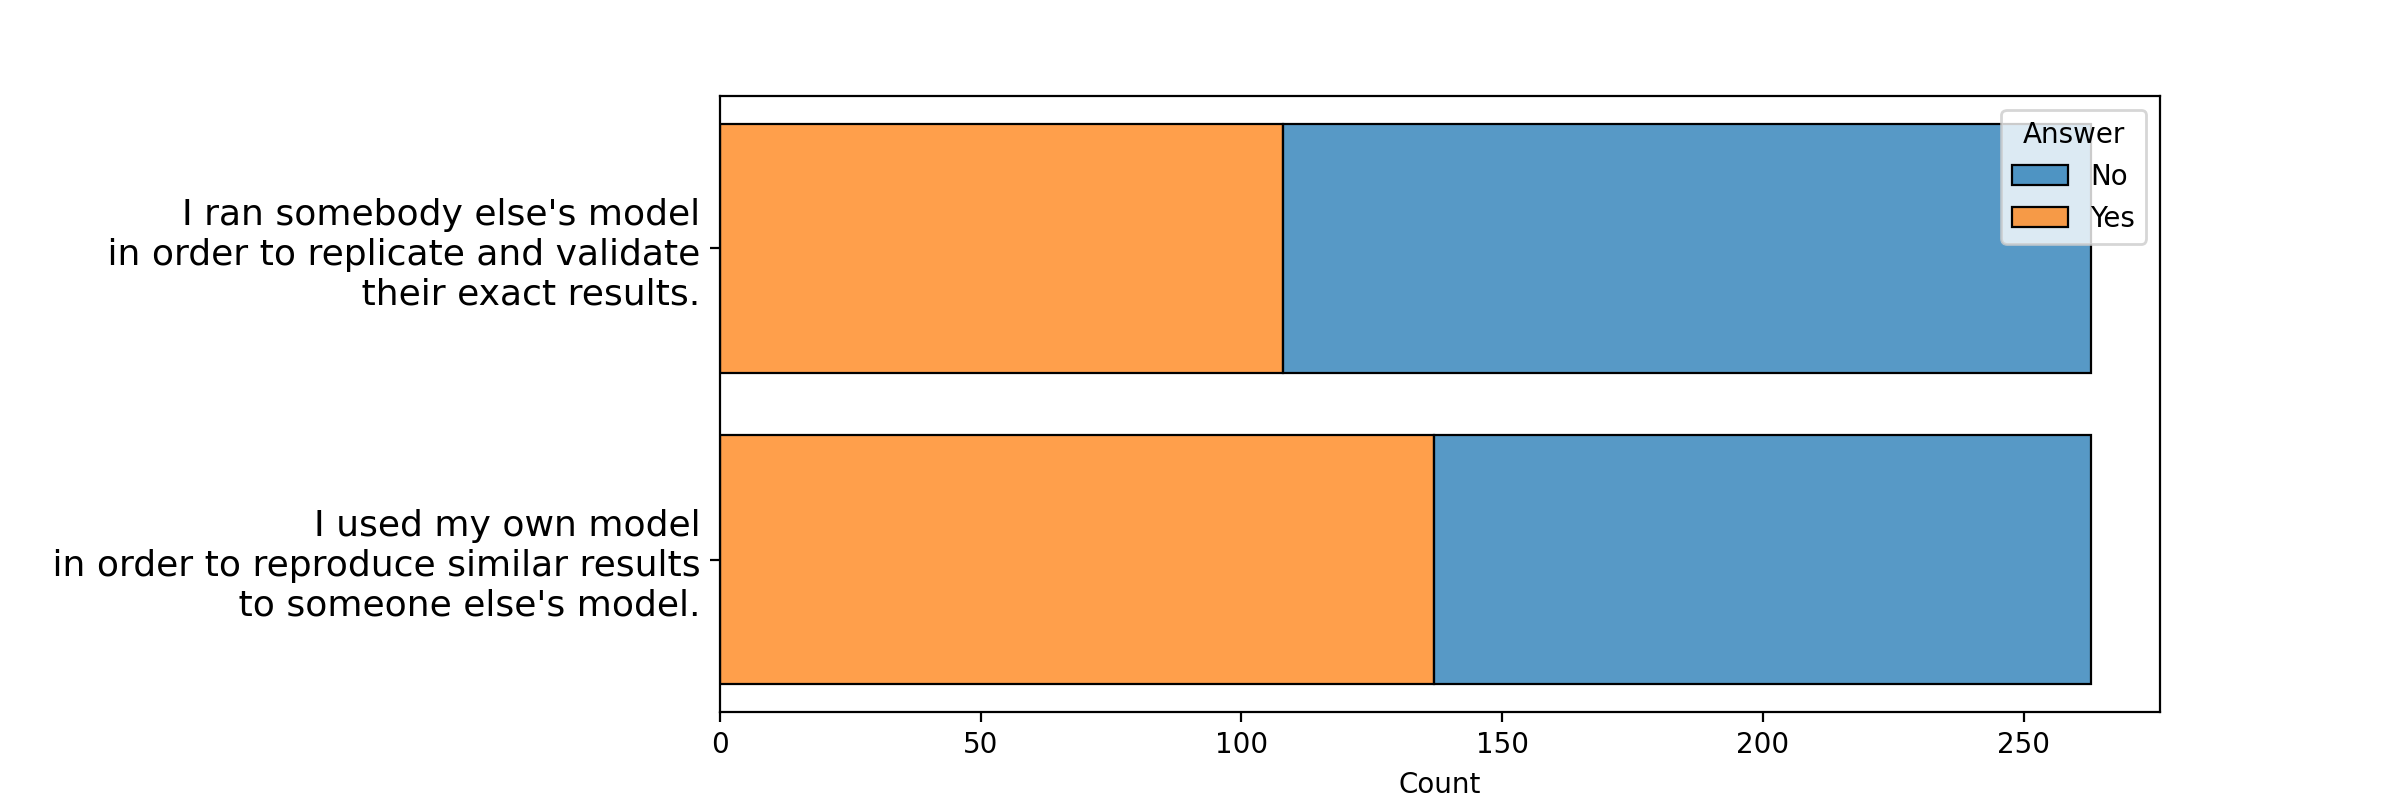
\includegraphics[width=\textwidth]{../figs/O102.png}
	\caption{O102 Did you reproduce results?}
    \label{fig:O102}
\end{figure}

\begin{figure}[!p]
    \centering
    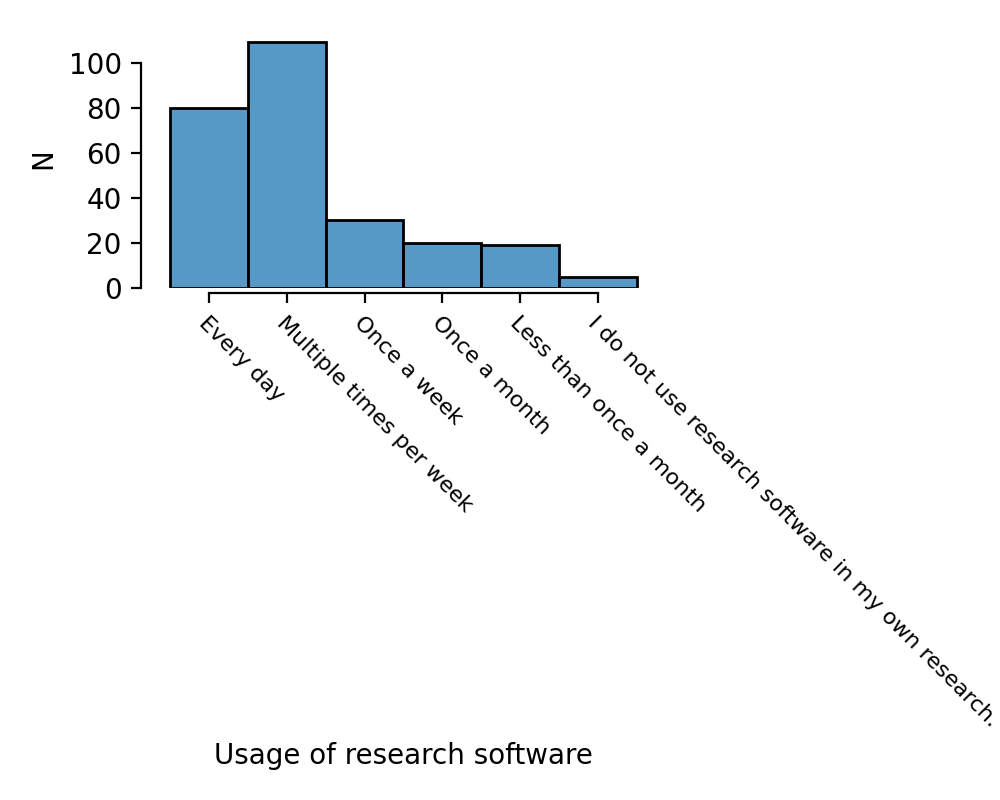
\includegraphics[width=\textwidth]{../figs/S103.png}
	\caption{S103 Frequence of using software.}
    \label{fig:S103}
\end{figure}

\begin{figure}[!p]
    \centering
    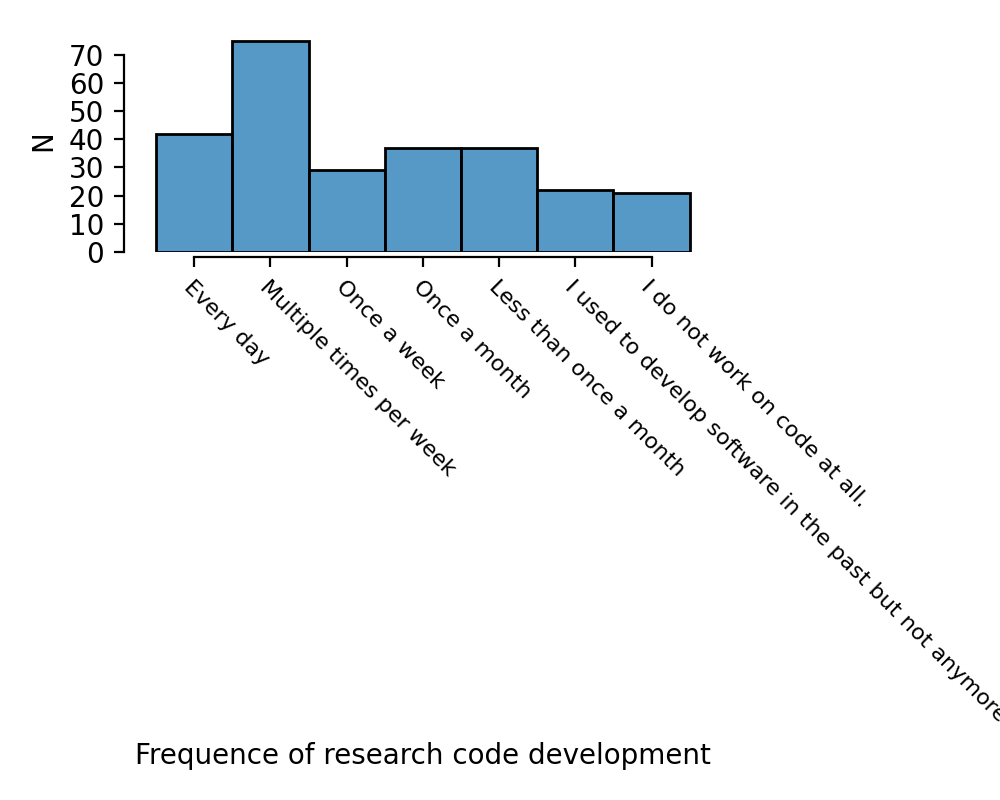
\includegraphics[width=\textwidth]{../figs/S110.png}
	\caption{S110 Frequence of developing software}
    \label{fig:S110}
\end{figure}

\begin{figure}[!p]
    \centering
    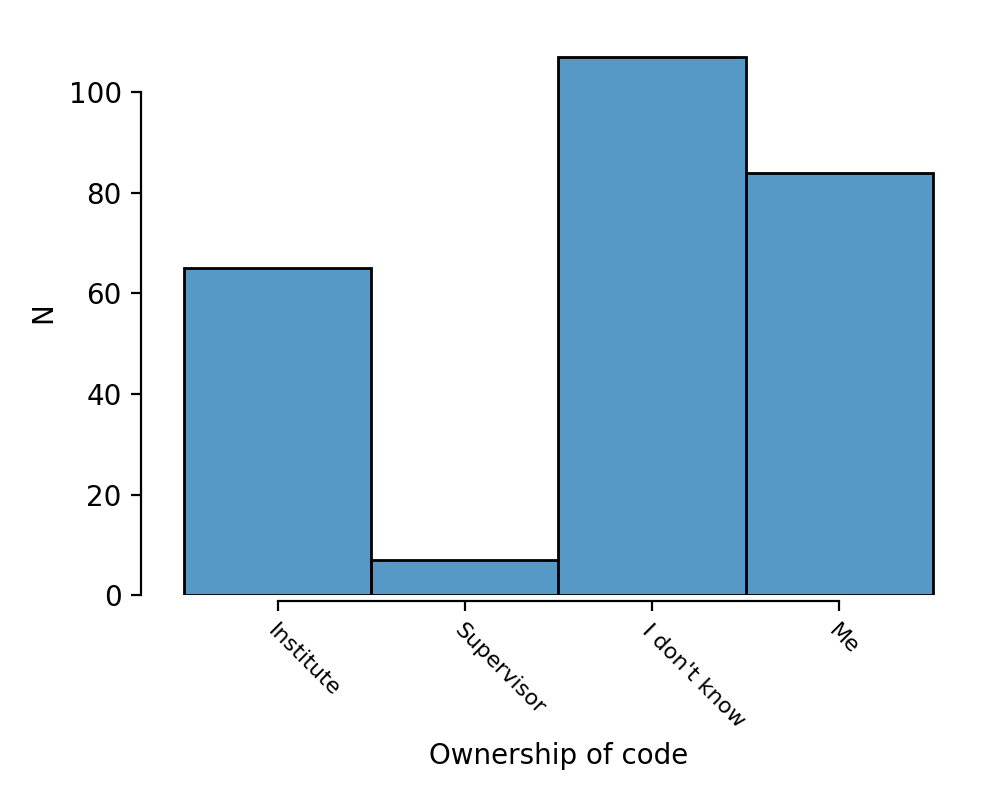
\includegraphics[width=\textwidth]{../figs/S202.png}
	\caption{S202 Do you own your software?}
    \label{fig:S202}
\end{figure}

\newpage
\subsubsection{H6 Knowledge}

\begin{figure}[!p]
    \centering
    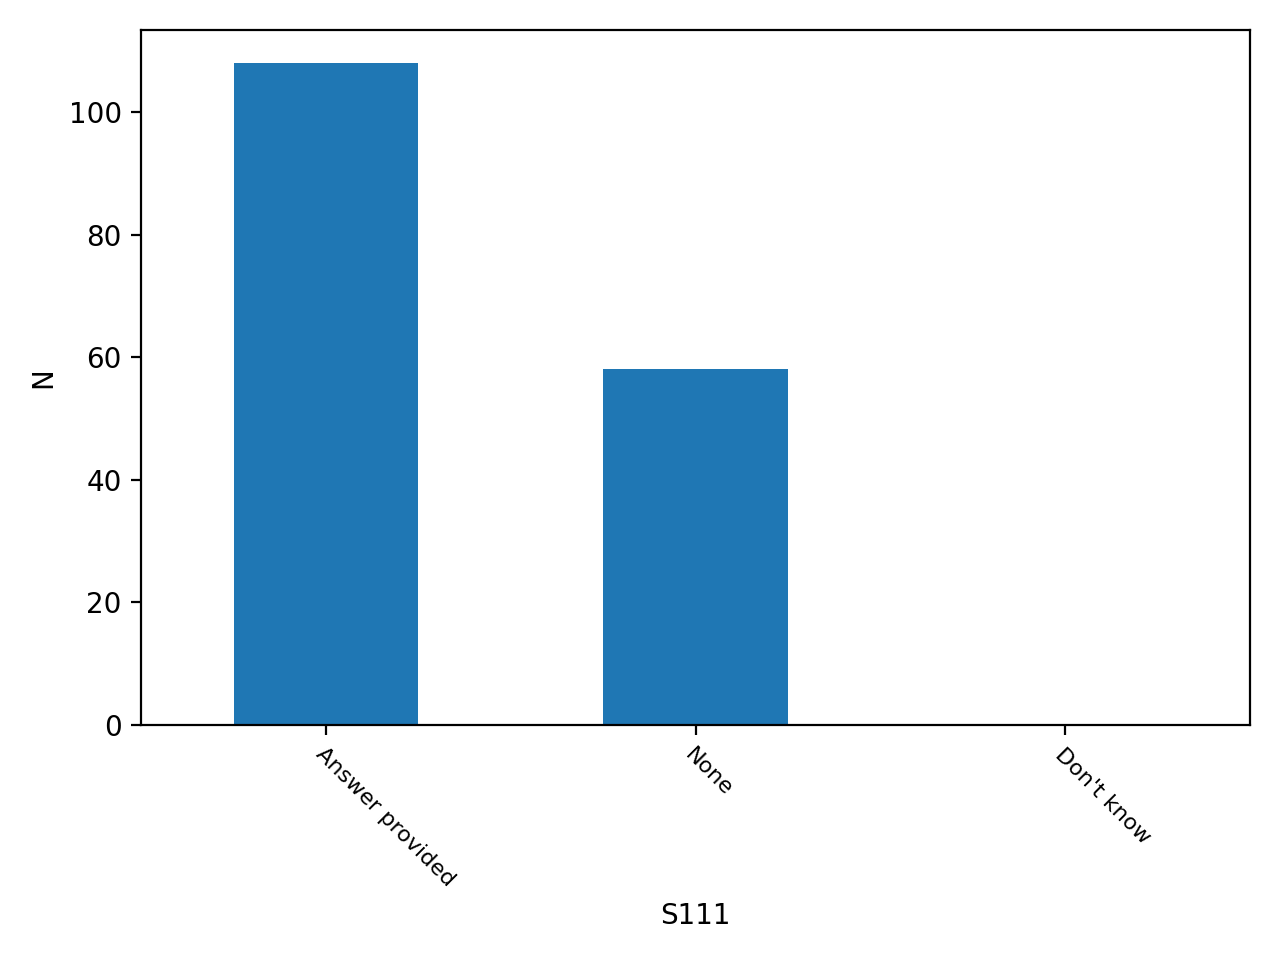
\includegraphics[width=\textwidth]{../figs/S111.png}
	\caption{S111 What software license are you using? }
    \label{fig:S211}
\end{figure}

\begin{figure}[!p]
    \centering
    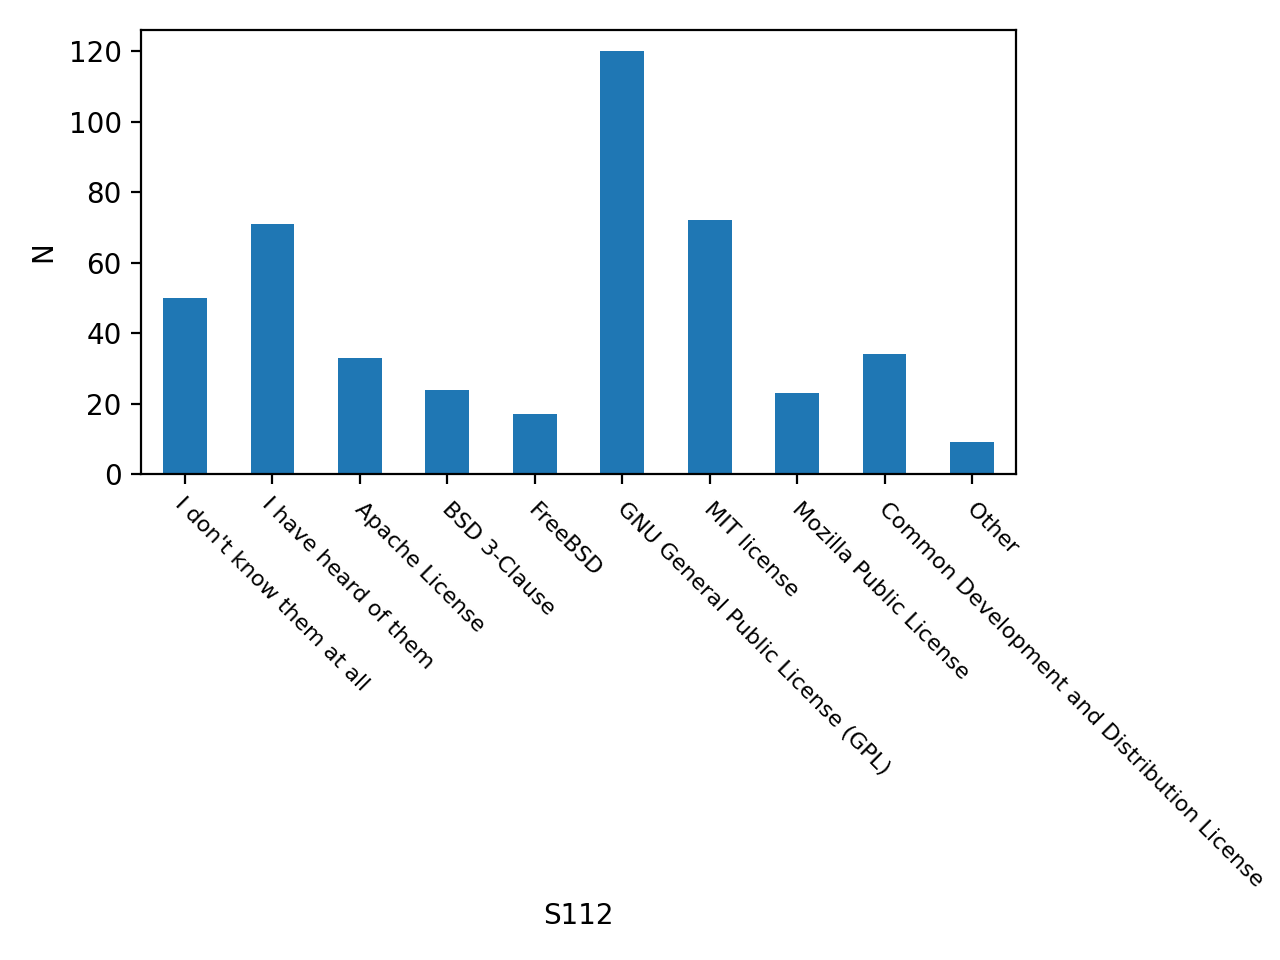
\includegraphics[width=\textwidth]{../figs/S112.png}
	\caption{S112 Which licenses are you familiar with?}
    \label{fig:S112}
\end{figure}

\begin{figure}[!p]
    \centering
    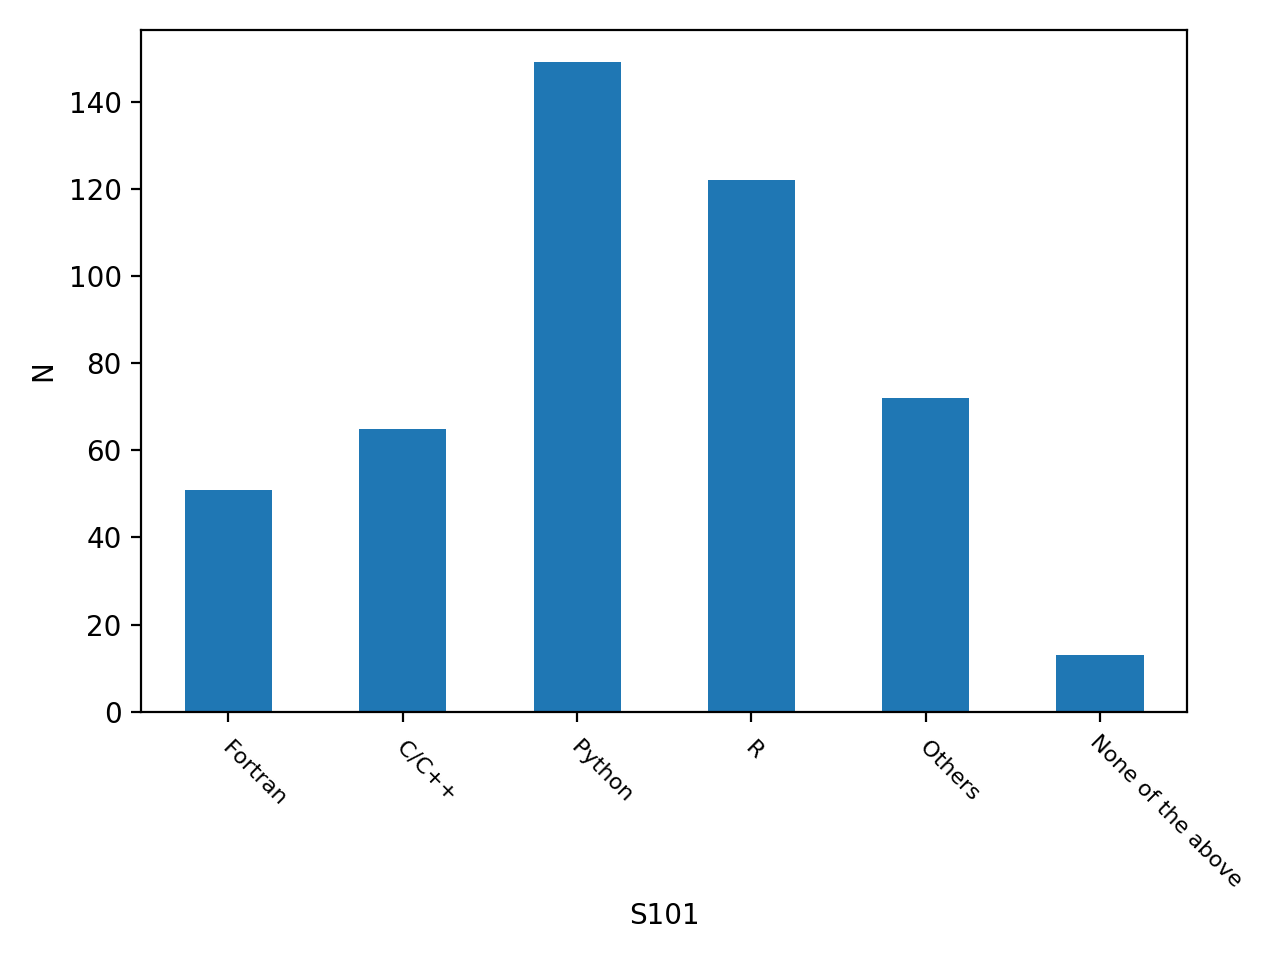
\includegraphics[width=\textwidth]{../figs/S101.png}
	\caption{S101 What languages are you using?}
    \label{fig:S101}
\end{figure}

\begin{figure}[!p]
    \centering
    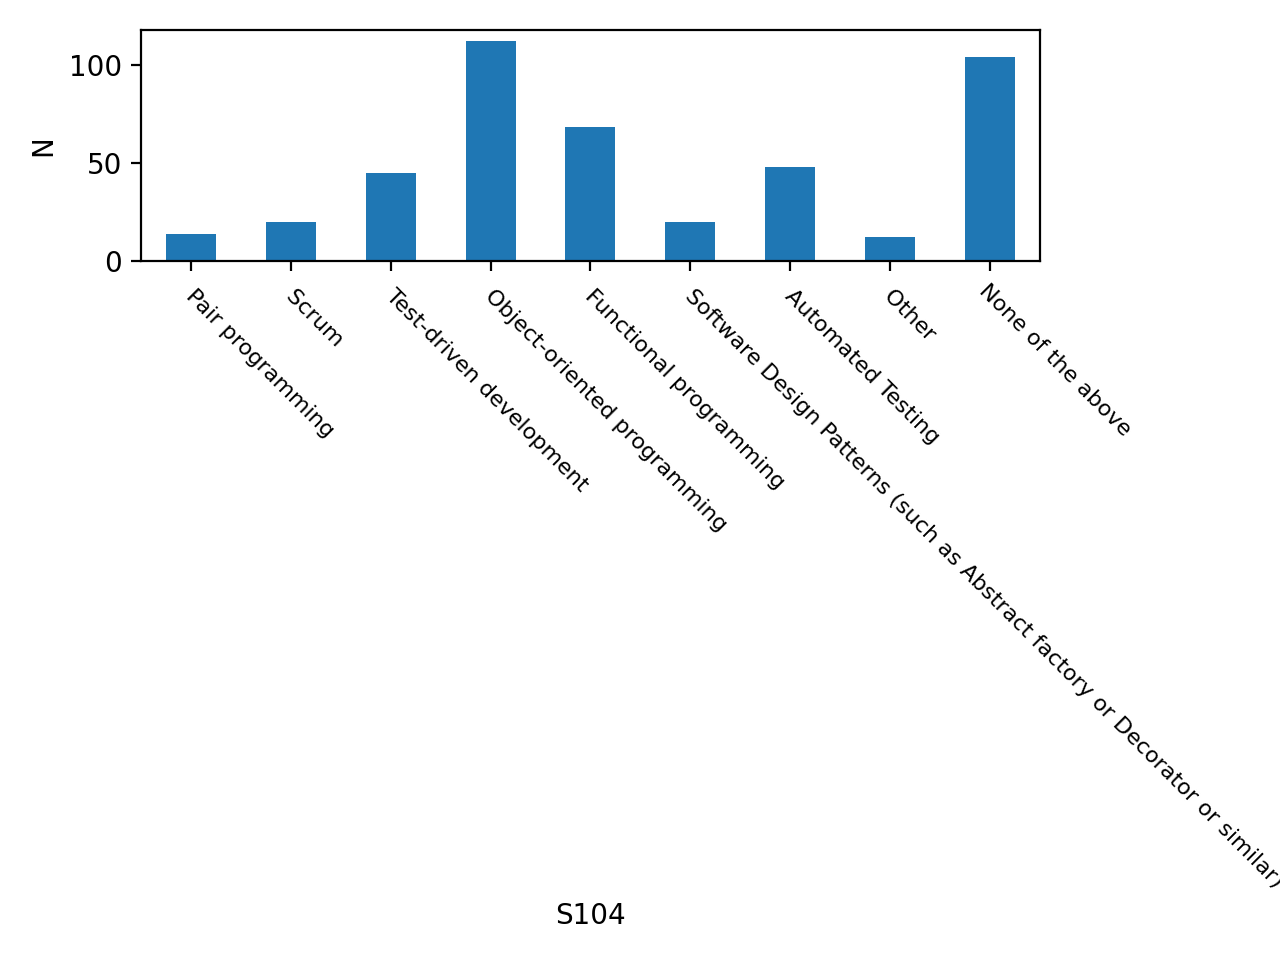
\includegraphics[width=\textwidth]{../figs/S104.png}
	\caption{S104 What methods are you applying?}
    \label{fig:S104}
\end{figure}

\begin{figure}[!p]
    \centering
    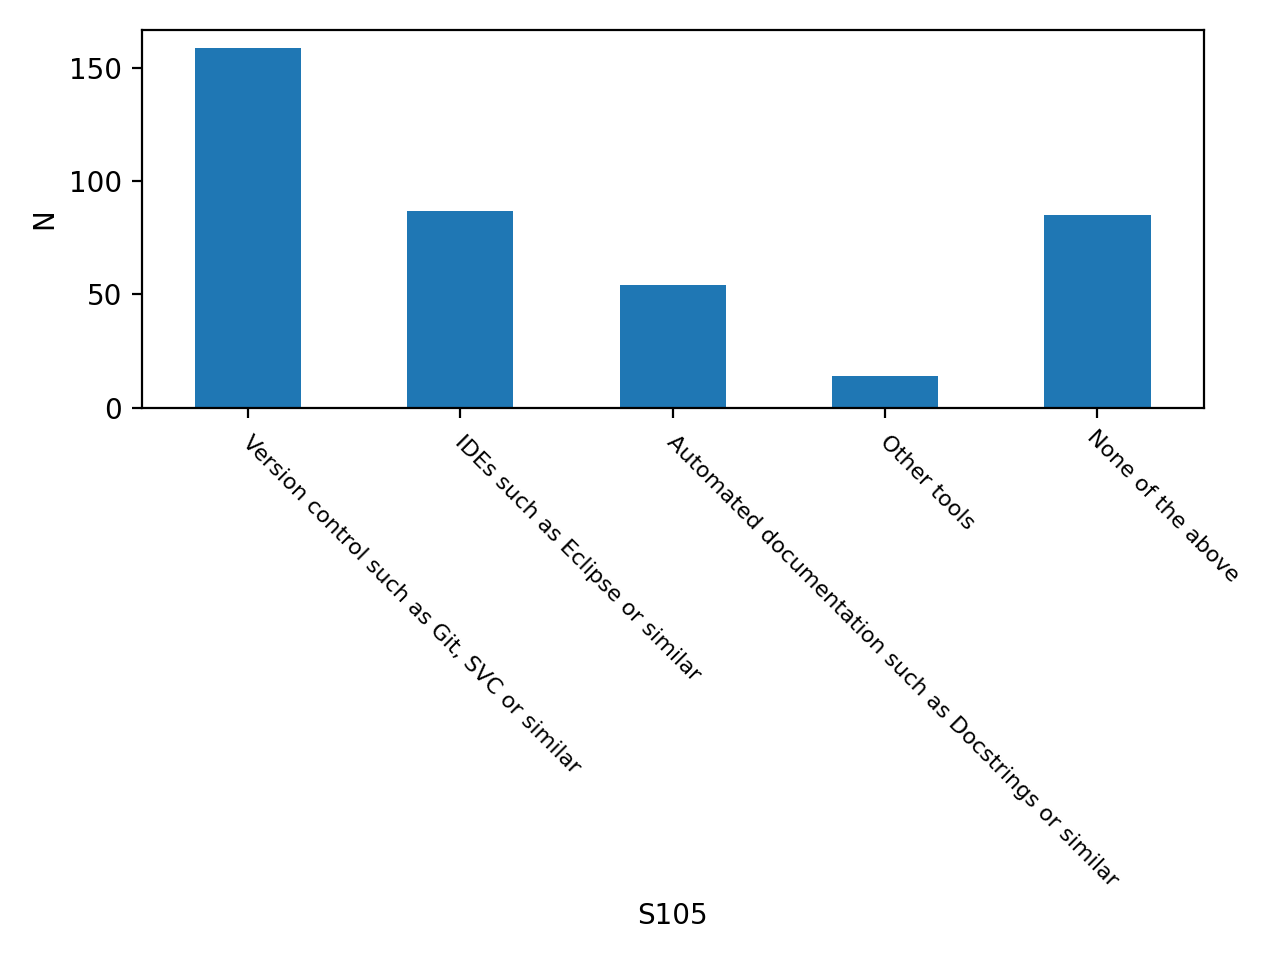
\includegraphics[width=\textwidth]{../figs/S105.png}
	\caption{S105 What tools are you using?}
    \label{fig:S105}
\end{figure}

\begin{figure}[!p]
    \centering
    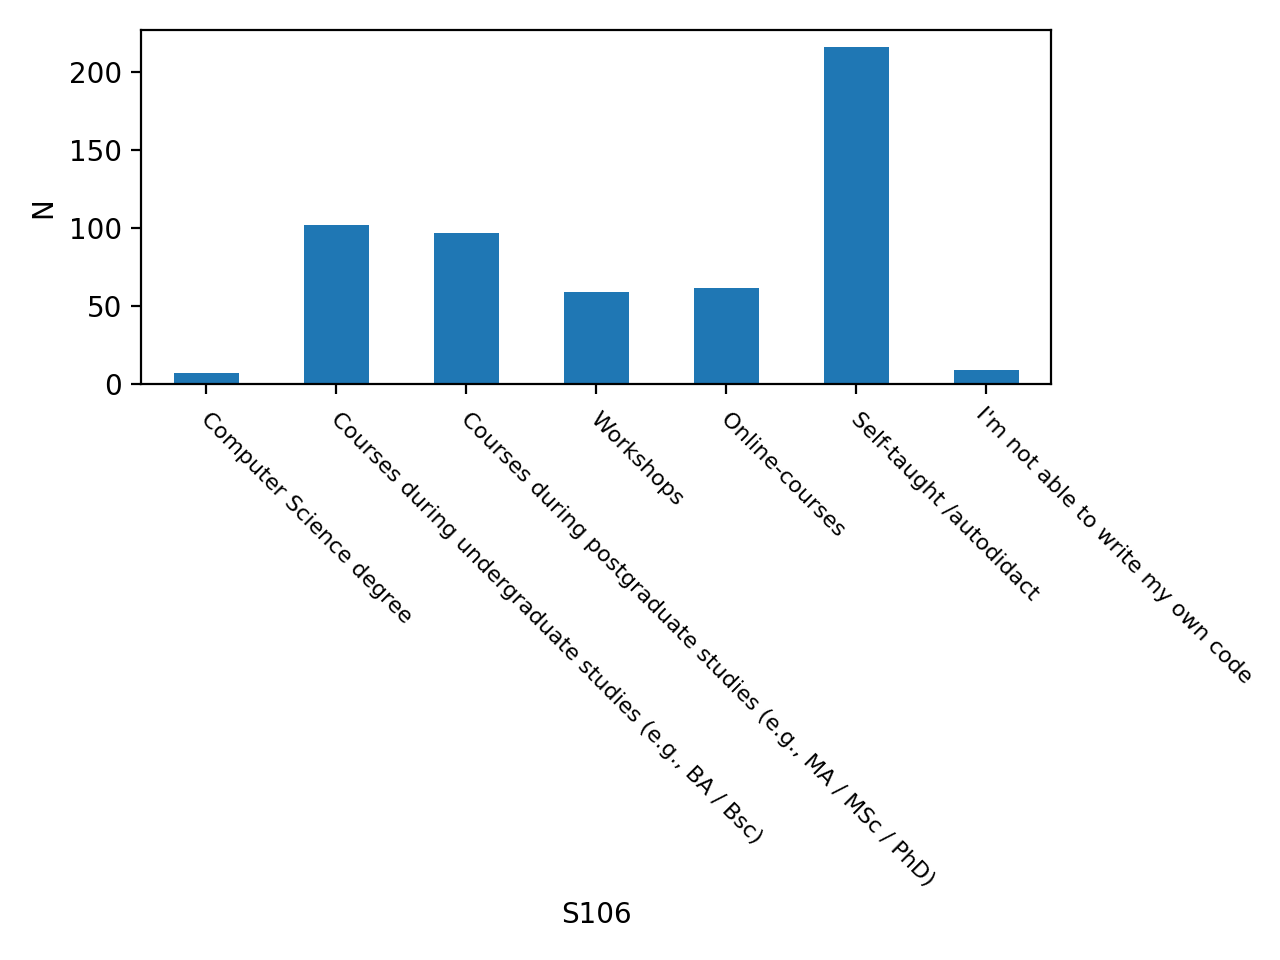
\includegraphics[width=\textwidth]{../figs/S106.png}
	\caption{S106 What training do you have?}
    \label{fig:S106}
\end{figure}


\newpage

\textbf{S111}

What software licences do you use? Results: [None 'none' 'hfvjhgjh' 'GPL' 'MIT' 'Creative Commons'
 'CECILL-C Licence (a French equivalent to the L-GPL licence)'
 'Creative Commons licenses' 'None' 'MIT, LGPL' 'MIT / GPL3' 'GPLv3'
 'Creative Common' 'GNU' 'Apache License v2' 'GPL MIT' 'GNU GPL v3'
 'MIT license' 'CC BY-SA' 'Apache License' 'BSD' 'mit' 'GPL, PD, WTFPL'
 'MATLAB' 'GNU General Public License (GPL)' 'Gpl v3' 'GPL, MIT' 'CC'
 'mit, ah hoc' '???' 'GPL, MIT, Apache'
 'GNU General Public License (GPL), BSD 3-Clause' 'Apache 2.0'
 'US Government work - Public Domain' 'NONE' 'BSD 3-Clause' 'GPL3'
 'Apache' 'FreeBSD' 'SWMM' 'BSD, GNU' 'GPL or CC-4.0 non-commercial'
 'BSD 3-Clause, MIT' 'GNU 3, MIT' 'MIT, GPL' 'GNU GPL' 'educational'
 'MIT, GNUv3, Creative Commons' 'GNU General Public License'
 'MIT, GPL, or commercial (depending on use)' 'MatLab' 'BSD3, GPL'
 'GPL v3' 'NOne' 'BSD-2-Clause License' 'GNU LGPL-2.1 License' 'MIT, BSD'] 
\textbf{S112}

Which of the licences are you familar with?

Other licences mentioned: [None 'CC0, Unlicense, WTFPL' 'LGPL' 'PD, WTFPL' 'None' 'Creative Commons'
 'ArcGIS, Django' "ESRI's ArcGIS" 'MatLab' 'MIT']
\textbf{S101}

What kind of programming languages do you mainly use? 

Other languages mentioned: ['Matlab', 'MATLAB', 'NCL', 'GAMS', 'matlab', 'ECMAScript', 'bash', 'Java', 'MatLab', 'Linux bash', 'shell', 'MPI', 'Stella', 'OpenFOAM', 'Delphi', 'PERL, MatLab, Pascal', 'Bash', 'Legacy (meta) languages in MS Office and ESRI: VBcode, AML (1981-1999), model builder. TBX ', 'Matlab and if possible I try to provided also compiled versione for complete reproducibility', 'whatever the students want to learn and /or makes sense for a particular project', 'Basic', 'Matlab, Julia', 'Octave/Matlab', 'Julia', 'Matlab, IDL']
\textbf{S104}

What methods are you applying?

Others mentioned: [None 'Procedural programming' 'UML' 'Continuous Integration'
 'Validation by comparison of numercial results with analytical solution or code-to-code intercomparison'
 'None' 'Yelling at machine'
 'git reviews with other researchers on the same project'
 'continuous-integration' 'Maybe?' 'team code review'
 'Open-source development (issues / pull-requests on GitHub, GitLab, etc.)']
\textbf{S105}

What tools are you using?

Others mentioned: [None 'Pycharm' 'Automatic formatting; issue tracker'
 'ReadTheDocs/TravisCi/PyCharm/GitHub/' 'Doxygen ' 'Code quality Checkers'
 'Markdown' 'Continuous Integration tools: TravisCI, CircleCI'
 'Cloud drive storage such as Box to maintain an archive of previous versions'
 'No'
 'jupyter hubs to make sure all members of the team work on the same distribution'
 'Autoformatters, Pre-commit hooks, Test Coverage, ' 'Jupyter notebook'
 'auto-formatters, linters, test frameworks, continuous integration tools'
 'Continuous integration']\textbf{S203}

What keeps you from publishing as Open Source?

Other reasons mentioned: [None "I don't write code"
 "I publish my code in out institutions library network, which can be freely accessed, but I'm not sure if this qualifies per se open source."
 'The model I am developing is not mine and the owners do not want to make it open-source. '
 'Code is unique for a certain data set. '
 'code not ready - still in development phase'
 'I try to publish most, but often time is lacking to bring it into a shape that it can be used by anyone (all bugs checked, properly documented)'
 'if possible in terms of time, codes have been published'
 'Too shy, worried about code quality' "Haven't published any yet"
 'I don?t know if it would be useful'
 "Haven't come to completion of PhD projects yet, but I plant to make everything open source"
 'not good enough to publish' 'Supervisor opposition '
 'The exceutable files are available on the web as a package that is regularly updated'
 'most of software has been developped during non-paid time and/or for personal consulting purposes. Some concern on giving away "for free" all of this immense invested non-paid time. Further, my code is relatively simple.'
 'LPJ-GUESS model that we frequenctly use is not openly licensed by the main development group in Lund.'
 'sensitive data/privacy and legal issues'
 'I have not spent a lot of time thinking about the subject, but I do publish my code on github'
 'Priority. I publish open data... I publish maps... I include scripts/code in some datasets... For others, it is so legacy format, that I archive it privately. '
 'not sure how and what are the standards' 'No specific reason']



\newpage
\subsubsection{H9 Activity of reproduction}
See also Fig. \ref{fig:O102}

We mainly have answers from hydrology. Splitting and plotting the results proably wont get much additonal information that is valuable. Core for plotting this is implemented in the plotting script.

\subsubsection{H12 Software ownership}
See Fig. \ref{fig:S202}.

\subsubsection{H2 Licensing}
Number of younger researchers which do not know about licences: 101

Number of established researchers which do not know about licences: 17



\subsubsection{H7 The most frequently used language}
See Fig. \ref{fig:S101}

\subsubsection{H13 Models that are available are hard to use}
Not possible to clearly answer this question.

\subsubsection{H3 Young scientists are more familiar with modern development methods}
Younger = less than 20 years of experience. 

Number of younger researchers which do not know about methods: 86

Number of established researchers which do not know about methods: 18



\newpage

\subsection{Hurdles against and Solutions towards Reproducibility}
In this part we are assessing what keeps scientists from publishing as Open Source and what we can do do increase reproducibility.
We expected to see lack of funding as mean reason and a main solution to the reproducibility problem.


Corresponding hypotheses
\begin{itemize}	
	\item H19 We need more funding to enable reproducible computational science.
\end{itemize}

Corresponding survey questions:
\begin{itemize}
	\item S203 - What keeps you from publishing as open source?
	\item S201 - What would help to increase reproducibility?
	\item S204 - Open text - what can the community do?
\end{itemize}

\begin{figure}[!p]
    \centering
    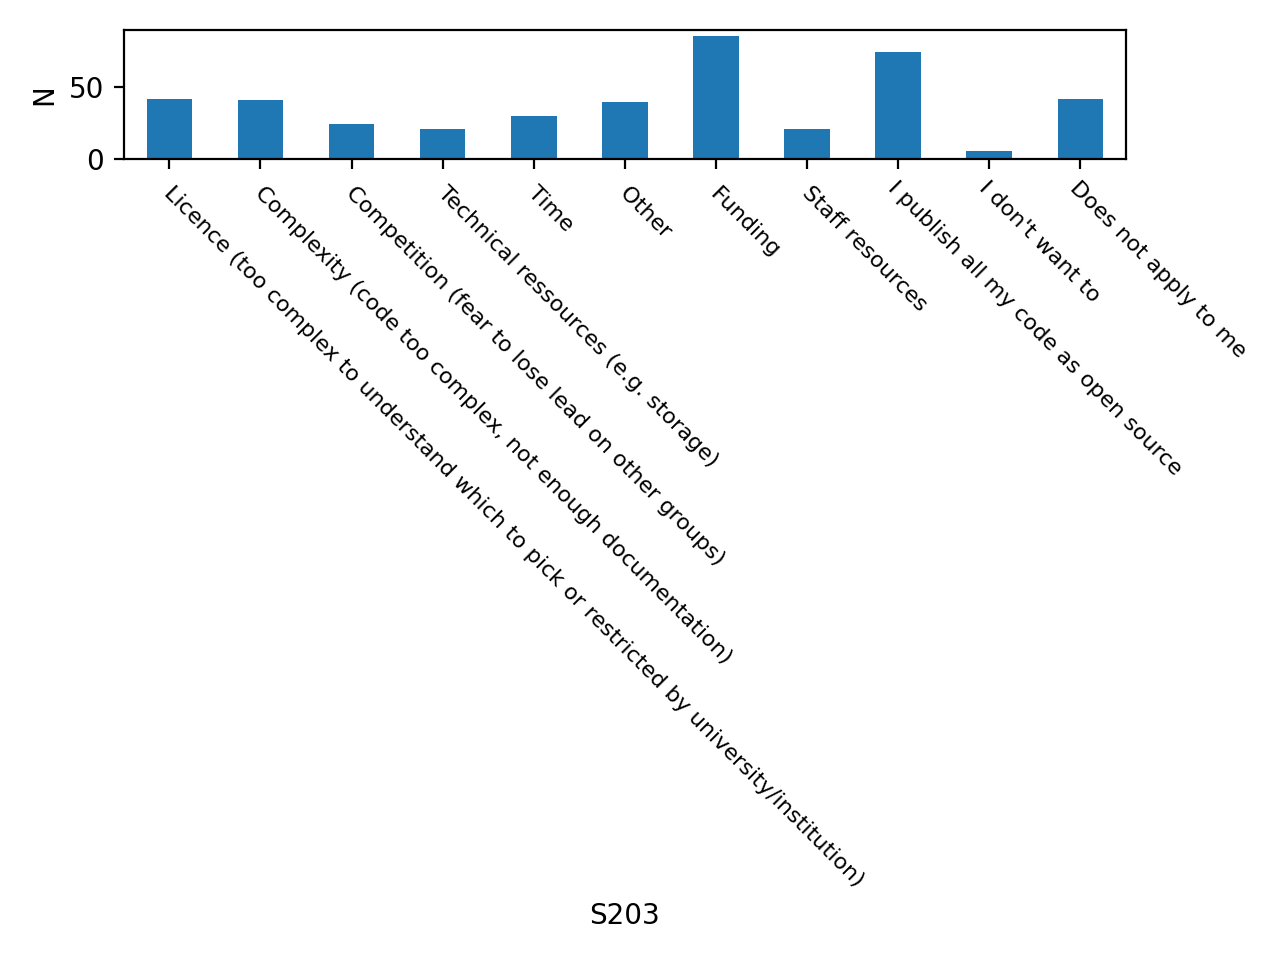
\includegraphics[width=\textwidth]{../figs/S203.png}
	\caption{S203 What keeps you from publishing as Open Source?}
    \label{fig:S203}
\end{figure}

\begin{figure}[!p]
    \centering
    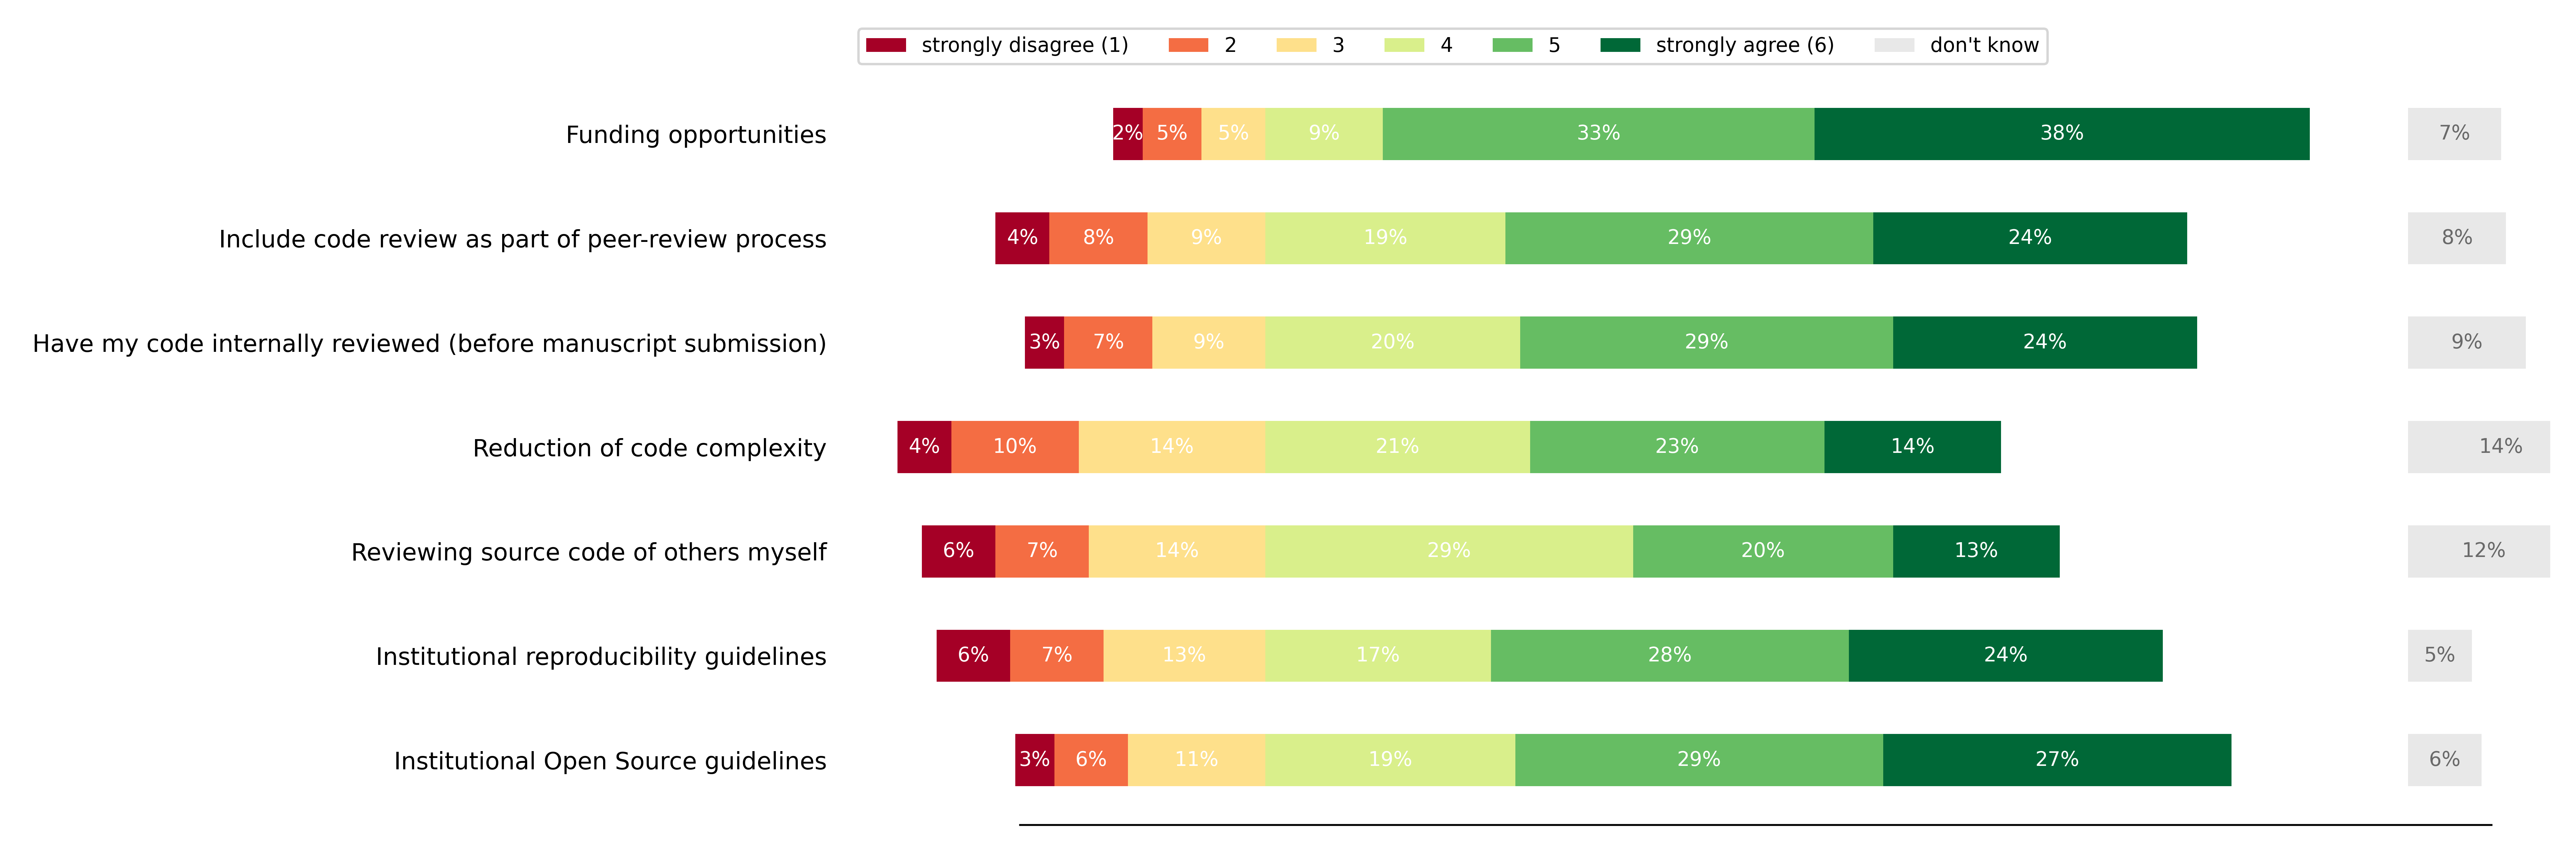
\includegraphics[width=\textwidth]{../figs/S201.png}
	\caption{S201 What would help to increase reproducibility?, First question mean is at 4.95}
    \label{fig:S201}
\end{figure}

\subsubsection{H19 Funding necessary?}
See Fig. \ref{fig:S201}

\newpage

\subsection{All fulltext answers}
This is a manually cleaned collection of the full text answers.
If you would like to access the uncleaned data use the S204.csv file.

The follwing organizes the answers into overarching ideas that were suggested. If an answer suggested multiple ideas it was split. But no content was removed!

\begin{figure}[!h]
    \centering
    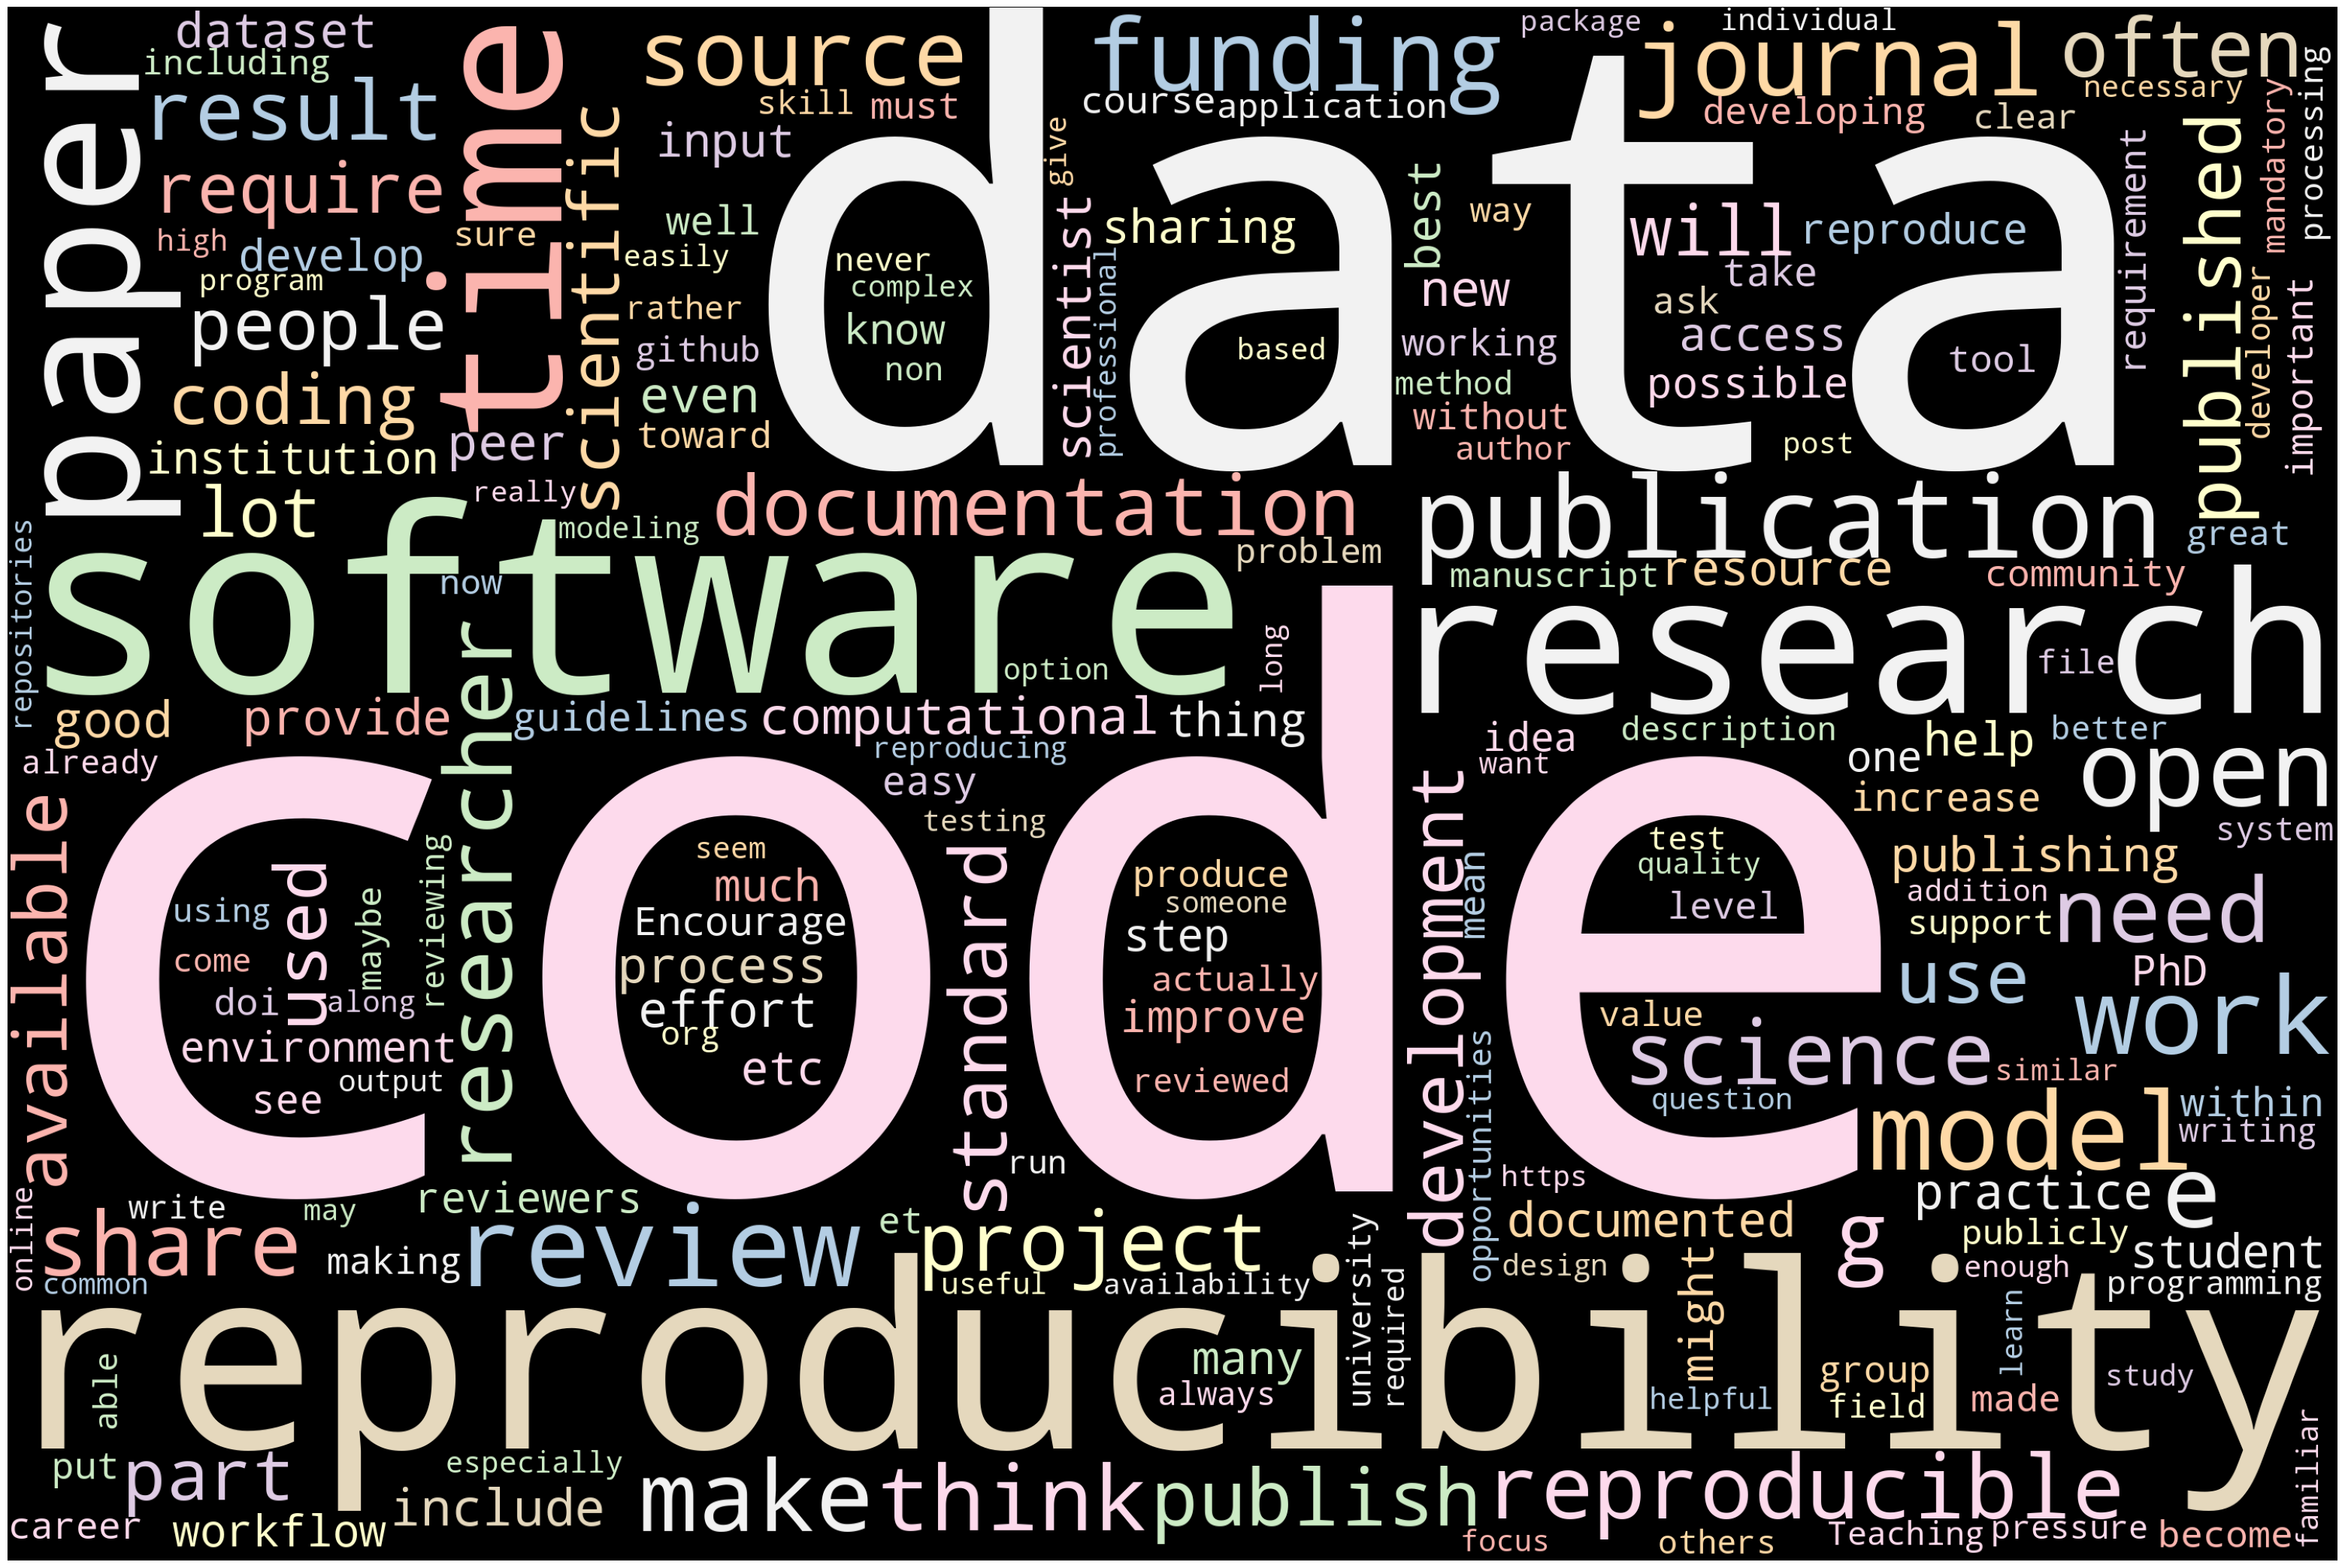
\includegraphics[width=\textwidth]{../word_cloud.png}
	\caption{Full text answers as word cloud.}
    \label{fig:wc}
\end{figure}


\paragraph{It is complicated}
\begin{itemize}
	\item In the climate community this is not very easily addressed. Reproducing the output of global climate models would be absurdly time and resource consuming. Reproducing the paper figures based on the author's code and data used is doable, but is it complete reproducibility?
	\item The emphasis of reproducibility and novelty is killing sciences in the developing world, especially in over-exploited complex GW systems.
	\item I am overwhelmed with the endless variety of licenses, programing languages, sharing repositories, the constant migration towards newer approaches that make older ones obsolete. I don't know how to, but if this could be streamlined it would be most useful to me. The community would need to agree to some standard sharing norms that we all should follow.
	\item Thanks for taking up the idea. Really important  issue. However for me reproducibility in modelling in hydrology would not mean just coding issues, the questionnaire is a bit biased toward formal criteria concerning coding. Reproducibility of research in mathematical modelling (including statistical models) in   hydrology is a  more complex issue.  I doubt, that even being offered the codes, all raw data and a detailed  description of the work done, it would be easy to reproduce someones results nowadays. These include subjective interpretations  of partial results and decisions taken based on these. Hydrology is not a lab science.
	\item I am not so sure that in our field reproducibility MUST be a condition for publication. It is not only a matter of considering the code. It works with data, which, depending on several circumstances, might have been acquired to a very high cost in financial and physical terms. Sharing this data might have certain non-convenient related aspects. For instance, multiple analyses might be associated to a unique data set. Writing a manuscript, depending on job-related conditions, may take a while. In the meanwhile, between a published work instant, some other research group might be working with ""your"" data and publish one of your ideas, before you, who actually collected the data; all of this, just because for publishing your past research you were obliged to share all of your data and code just because of ""reproducibility"". Further, it is my oppinion that ""doubting"" on our research results just because we do not share everything, including software and data, is not that  correct, nor that logical. Shall we doubt on what has been already published?... on the work of Beven, Refsgaard, Abbot, etc (hydrology)? Beven have shared TOPMODEL, most probably becasuse he was always interested in so, but al;so because its original development was financed explicitly with that purpose in mind... The Danish effort of Abbot and Refsgaard, MIKE SHE, is commercial... what will happen when I do research with a commercial software and cannot share it... even if I share the data, the research won't be 100\% replicable.... does it mean that the research is bad and as such non-publicable?
	\item Funding dedicated to this would be great. Stricter requirements (e.g., code review with publication) could be useful, but I worry about unintended consequences and the practicality - e.g., might become more difficult to find reviewers, more difficult for early career researchers in computational fields to publish relative to competitiors in non-computational fields.
	\item recognize that just sharing the code does not gaurantee reprodicibility. Results are very dependent on libraries used, often even operating systems used (famous example where MRI results were treated differently on mac vs windows machines in genetics research because the file sorting algorithm was different for those operating systems)

It is therefore 
- important to consider the entire compute environment used when working towards fully reproducible results
- try to keep this compute environment as lightweight, portable and machine agnostic as possible. Currently containers are a great way of achieving this.
	\item The COMPLEXITY of reproducibility is often underestimated. This issue has been a major topic within the social sciences, and there now exist a nice collection of resources that necessarily reflect the broad range of what is considered ""reproducible"" and there are insights and resources portable to the geosciences, see e.g. https://www.bitss.org/
\end{itemize}

\paragraph{Share more and share data and model together}
\begin{itemize}
	\item Foster putting codes publicly available (e;g. through github)
	\item Share not only model, but when using application: (1) Share the input and settings you have used to run the model. Share (if possible) the dataset that you have used to compare the simulation results with (when comparing simulations with real data).
	\item Publish data alongside research papers. With the documentation contained within the paper, the results should be reproducible.
	\item Publication of code and (exemplary, applied) data with the manuscript as a standard ? but also acknowledging the extra efforts required for this.
	\item A more detailed description in the paper and a share option for code "share code and data with others, stronger collaborative efforts rather than competitive mindest, reduce the amount of code developing by individual working groups and rely more on available codes and community efforts for code development for similar questions and applications.
	\item develop and maintain open access databases
	\item Agree on common tests for code, models.
	\item Make data and code publicly available and thoroughly documented
	\item SHARE! Share your data, share your code!
	\item Improve sharing culture of open access data - data is often the problem
	\item Models needs data and produce data. data should go with the FAIR priciples
	\item Providing step-by-step supporting information besides the results. Listing all the assumptions.
	\item Encourage publishing of code online in repostries like github.
	\item One challenge that I see with reproducibility is the need for openly accessible data. Individuals who fund field campaigns that generate data feel somewhat ""used"" by modellers who do not obtain funding to generate data and in some cases expect that all data should be freely available. Essentially, if one researcher goes through the trouble of collecting and funding data why should the rewards of their efforts go to others before they have had the opportunity of fully exploiting that data. Additionally, if you put a temporal embargo on data availability so that data is private for some duration this may prevent students or PIs from publishing findings involving that data within that time period because of journal data sharing requirements. Perhaps using synthetic data is an option for demonstrating analysis and validity without exploiting data generators.
	\item It's not only about codes but also about data which should be published along with the code. I think the past decade has seen some progress in making codes publicly available.
	\item Show your work in appendix, attachment, online, etc
	\item - We need to have an honest discussion about why people don't share their code. My impression is that the answers are similar to why anonymous reviews should be maintained.  
- Researchers are rarely required to produce good code. I mean when was the last time someone took your code apart and tested it? And producing good code takes practice, but also the need to want to write well-structured and well-tested code. I think the problem can only be improved if we accept that all of us are part of it and that all of us probably produce research output that is not reproducible.
	\item Share codes or softwares but overall share the input files. Do not publish papers that relying on code and data do not provide them. Stop using proprietary close-source software. Ever.
	\item The models that we use need to be open-source. Also, sharing the scripts (e.g. via GitHub) that we use for data post-processing would be useful and maybe even necessary.
\end{itemize}

\paragraph{Check during submission and journal responsibilities}
\begin{itemize}
	\item Most data are already provided within the most publications. So why not using a software tool during the submission to check reproducibility of results based on the code and the data
	\item Journals should enforce FAIR not just get everyone away with it
	\item Submitting for publications and working on open source codes could be made the norms by the editors.
	\item code repository connected to scientific journals where the modelling study is published
	\item Publishers, Editors, and Reviewers should require all source code to be made available in open repositories (if necessary with a restricted access like Zenodo)
	\item Increase mentions of code sharing and research reproducibility in research publications, include code review in peer-review process.
	\item not accept papers anymore that obviously have something to hide or are completely unwilling to share.
	\item more critical peer review on methodology/code (when supplied as supplementary material, no review is required/possible) 
	\item When reviewing a manuscript (mine or other), I ask myself, can I make the same model from the information in the code? Are inputs explained? what assumptions were made? Making these things very clear can help. 
	\item I would love to discuss how to standardize reporting model setups. I think this should probably rather come from journals.
	\item Include all codes during publication of work, should be mandatory by all journals.
	\item Move beyond the static paper and encourage to have the code as supplement, or do things like jupyter notebooks in addition or instead of a paper.
	\item Encourage / demand data and software to be published along with research papers. Strengthen the role of peer-review (e.g. stronger acknowledge Publons) and post-publication review (see Pubpeer).
	\item A big help would be to have code available as frequently as possible and it being part of the review process. Datasets should be easily made available. When those cannot be shared, present synthetic series and results to be replicated by the community.
	\item only reproducible Research for publication
	\item Include more code in papers and describe it Better/required documentation
	\item Journals should mandate reproducibility and include it in the review process.
	\item We are moving towards the right direction. Code should be attached to publications along with ALL input data and the reviewers should be able just to run it to see if it works, if it generates the same outputs presented in the paper and eventually to check if all steps are correctly implemented.
	\item Just share the code with good documentation and comments. So many high impact journals have no code documentation at all (even recent ones, despite apparent journal requirements). There is a huge burden of time for researchers to do this, though.
	\item Impose to publish with open source model codes
	\item Every paper should provide code and data for running and plotting every figure in it.
	\item A reproducibility-test should be part of the review-process. 
	\item Encourage code releases or links to source-code repositories as part of the manuscript acceptance/publication process, similar to how data is now commonly required to be released. There also needs to be an acknowledgement of the importance of releasing code in funding opportunities, and specific funds allocated for that. 
	\item Move towards requiring all source code and data (that does not have legal restrictions on its use) to be published or deposited in a publicly available respository for all publications. 
	\item Journals should require code/data for publication where possible. Code review would be great, but it would probably be too time consuming for volunteer reviewers. Maybe journals could hire some data scientists to just check the code for correctness as a separate part of the review?
	\item Journals should move towards requiring experimental reproducibility as a part of criteria for publication.
This means abandoning the publish or perish model as a basis for professional advancement.
To enable this, collaborations to assess reproducibility should be professionally rewarded.
	\item Rolf Hut (yes, I know I broke annonimity...) ":
"Journals should push for open and reproducible code and open data. If researchers do not want to share their code/data, they should be able to give a good reason.
While clear guidelines are helpful, it should also be made relatively easy. There's already a lot we have to do as researchers, so there's limited capacity to also become a ""professional software developer"". I think being too demanding (e.g. as a journal) might put people off, so we should balance the requirements with the effort they involve. That's also true for reviewing. Code reviewing is generally a great idea, but it will make reviewing more time consuming. 
Then I think we should make a distinction depending on the type of paper/code. If it's a paper that presents a new model, for example, then I would require a more thorough code review compared to a paper that just uses that model to produce results. Generally, we should distinguish between research software, i.e. where the focus is on the software itself, and research that uses software. Well written and documented code is always helpful, but quite often specific code used to setup a model for a specific case study simply isn't reused that often. So I think it is potentially unnecessary to expect the same standards (e.g. documentation) in that case."
	\item enforce transparency policies with journals.
	\item ask for providing codes during article submission
	\item Require code to be published/available if it is used/referenced in a manuscript.
	\item Pay people who conduct peer review, and require reproducability be taken into account in the peer review process
	\item Put reproducibility as ""mandatory"" in the publication of our scientific results
	\item Make code publication mandatory, including working examples (at least small sample dataset). As witht he EGU copernicus journals, require data publication on some repository. If the latter is not possible due to data restrictions, require data repository of processed dataset (e.g. alternated values - same data disstribution and trend ...) and the entire post-processing workflow.
	\item Demand that the code is peer reviewed by qualified peer reviewers
\end{itemize}

\paragraph{Need for specialized personel}
\begin{itemize}
	\item We need people who can help to improve reproducibility, as many researchers with a focus on analytics and conceptualization are not familiar with coding and licenses. Still those researchers have great ideas that should not be ranked lower just because those people are not familiar with this new, necessary movement
	\item Invite experienced software engineers as consultants for model software development.
	\item Hire more research software engineers that oversee sustainable software development practices and help with standardising, testing, and publishing research software.
\end{itemize}

\paragraph{Teaching}
\begin{itemize}
	\item A lot of today's scientific endeavor is performed through a process akin to software development yet there is a blatant gap between the standards to which scientific code and industry code are held to. For the sake of reproducibility and as a service to many graduates that will pursue a career in the private sector, industry standards should be taught and enforced. Publishing code and data is not enough if the authors are the only persons able to make sense of it. Versioning, packaging, long-form documentation, testing, continuous integration and deployment should become widely accepted standards in scientific software development as they have become in the private sector.
	\item Teaching reproducibility (with respect to software, data and measurements) in environmental sciences.
	\item provide better material to learn about reproducibility and it's benefits, standardize the teaching of coding skills and their ""best practices"" in MSc or at the latest PhD programms, allocate TIME (and thus money) for making work reproducible
	\item Often clear guidelines and courses for beginners on how to ensure reproducibility from the very beginning are missing. For a beginner the different steps and tasks can seem overwhelming. Teaching from the very beginning and setting out the rules for a minimum standard could help improve the reproducibility.
	\item We need a lot more training. 
	\item Dedicate a few months at the beginning of a PhD or Postdoc position for a crashcourse in professional programming.
	\item Mandatory crashcourses for senior researchers and professors in how to *evaluate* code quality. If journal reviewers and supervisors have no idea what good software looks like, it will never be rewarded.
	\item Universities should teach how to increase computational reproducibility.
	\item Provide resources to help with the open science
	\item build on scientific code of others, and develop it differentially (in the sense of changesets).
	\item Give researchers the resources they need to learn to produce readable, well documented code and have consistent standards across journals regarding code and data availability.
	\item More classes at university level on coding and/or workshops for more advanced researchers
	\item Continous training is very important for aweraness creation.
	\item Include these concepts in courses taught to undergrads and graduate students
	\item There should be more courses on ""code documentation"" and ""publishing your code"" e.g. as public packages - not only at the university/institution level but internationally as well. From my experience, most people code for their own purposes, but they are willing (or even happy) to share their code, but they feel embarassed of its structure and functionality. To overcome this, they do not only need to learn the best practices, but also how to publish code; from small packages for simple tasks to complex packages for complex tasks. For the latter, often time to maintain these packages is lacking ? this should be accounted for somehow.
\end{itemize}

\paragraph{Practices}
\begin{itemize}
	\item Shadow or Pair computing could be made the norm.
	\item At my institution, we are lately developing a strong focus on reproducibility. Especially for young scientists who are starting their projects, e.g., PhD students (in particular those that come from a non-programmer background) this topic seems to be overwhelming. They are struggling to get familiar with the models, with programming, with their research projects, and they are now also asked to strongly focus on reproducibility, ideally to a level where they think about Continuous Integration, Conainerizing of models and scripts, and extensive documentation. This is a lot to ask of a beginner. What we often hear from them is that they are already severely time-constrained and would like to dedicate more time to reproducibility, but don't see how they can do it within their allotted time for their project/thesis. Reproducibility should become more of a standard procedure in modeling-associated research, but to actually make it happen, it seems that it needs to be planned into the design of the research projects right from the start, to ensure that there is enough time available that can be dedicated to make research reproducible, and to teach (young) scientists who are not yet familiar with the concept and the means to implement it.
	\item I would recommend reproducing the result by a colleague not part of the concerned project/paper before submission. I believe this will increase the confidence and reproducibility of the research. 
Communicate the workflow
	\item Require all code open source.
	\item Publish code as publication.
	\item Present your code to your lab mates, receive critiques
	\item Formalize the conceptual modelling steps prior to program coding
	\item Code review within my research group has been an incredible process for improving the readability, structure, and best practices of my code. Code review events or conferences might be a good way to improve reproducibility.
	\item Encourage standards / best practices for developing, documenting, and archiving code, including scripts for pre-/post-processing inputs/output data.
	\item Emphasize documentation, read-me?s. Transfer of information after someone finishes a PhD is so lacking because people are normally scrambling to finish, and don?t think to put their models in a shared drive
	\item Include the code as annnex to the manuscript with a clear description of the steps used to get to the presented results (i.e. imputs, paramenters type and values, followed procedure, exceptions, approximations...)
	\item All the inputs used for the computation must be rigorously described, and also the methodology for make sure that the produced results are correct (e.g.: convergence studies in CFD)
	\item The computational cost of replicating a global, continental, large-sample hydrological studies is too high. A sollution would be to create a demonstration dataset, which is a subset of the whole study, for testing reproducibility.
	\item Develop community standards for transparency and open-source softwater development (especially in the research community)
	\item Mostly an attitude  values thing. - Value publication of workflows and data similar to scientific findings - Encourage the citing of dataset/code DOIs (in addition to any papers describing said data/code) - Move away from the ""I needed time to create this code and I don't want others to benefit from my work"" attitude (by doing e.g. the two things above)
	\item Have more allocated time (i.e. and that relates closely to funding) to prepare codes that are relatively easy to read by others in order to be able to share them.
\end{itemize}

\paragraph{Institutional support and change}
\begin{itemize}
	\item The science community and funding institutions should put as high value on a good sceintific code - reviewed, documented and published - as on scientific papers. This actually also applies to research data that are along with software less valued than a paper. This requires a shift in a mindset which has started, but will take some time (years-decades) till we are there. You can do a PhD with three published papers, but not with a paper + a documented open-source code and a documented doi-Dataset! This is a point where to start change things. Of course, this may open door to easy-way PhDs consisting of a few subroutines, an Excel-Table and a low-profile paper, but this is what the supervisor and finally the PhD commission should look at.
	\item Universities should provide service entities which guide, support and review scientific software development to avoid the autodidact diversity of styles and mistakes.
	\item Universities should recognise Research Software (and related papers in journals such as JOSS) as publications and part of PhD theses. 
	\item Each institutions/university should make reproducibility a priority, create data bases like OpenABM website to upload open source codes.
	\item Guidelines for reproducible software generation, not just reproducible research in general, would be helpful, in addition to funding for improving established research software.
	\item Institutional know-how passing on and being updated. Organize within the institution. Create side projects within the institution where researchers can actually work and publish their code together. Make these side projects mandatory.
	\item Make reproducibility more understood by management and funding agencies
	\item Having an AGU or University wide standard to follow in our discipline would be nice as an early career scientist in order to follow best practices. 
	\item Offer more guidance and resources to groups from institutions.
	\item In my country (UK) there is very little funding for good coding practice and almost no professional incentives for such activities (i.e., reproducibility and production of open source software has never come up in an appraisal or promotion case for me). 
Maintaining software for the community is a lot of work and my employer would much rather see me write papers with that time. 
Universities like citations: more standarisation of software citation might change this balance of incentives. 
There needs to be more funding for research software engineers.
\end{itemize}

\paragraph{General change, time, funding, recognition}
\begin{itemize}
	\item Provide best practice guidelines, funding, and recognition for reproducible science. The current currency is publications, not well documented, tested, and reproducible research.
	\item I think that time is a very important factor. Many scientists work in projects that up to now often do not allocate time to the reproducibility process. So the time to invest in reproducibility competes with time to produce project results. I think it could help to actually allocate time (and thus funding) to making science reproducible in project proposals.
	\item And we need to acknowledge that this is a considerable time investment for PhD students and post-docs who are the main scientists developing code. Current projects have very tight timelines that are often not feasible because of poor planning and poor time management - this is without investing time in reproducibility. Time devoted to reproducibility needs to be factored into project proposals and projects need to be guided with a Scrum framework that allows scientists to quickly see what is working and what is not, and to promote working in teams (which would facilitate code review). A lot of coders and professors I know work as 'lone wolves' - but making code open source and reproducible will require us to help each other, work in teams, and promote a spirit of openness. Right now, no one in my project would have the skills to review my code. I would have to ask other lab members not paid by my project to do the work which is asking for a lot of time, especially since this person would not be familiar with the scientific goals of my model and the questions it is supposed to answer. Reproducibility is incredibly important and I think most people want to improve, but we need to be given the environment where we can make such a time investment. 
	\item Reduce publication pressure! Quality must come before quantity.
	\item Code and data publications should be treated as valuable as/equally to papers (including funding opportunities, best practices, peer-review obligation, importance for applications for scholarships/positions).
	\item funding for staff / coders in addition to funding for scientists.
	\item increase funding
	\item Common standards have to be checked regularly. Many manuscripts are published too fast...
My supervisor (habilitated years ago) often told me to do / code / calculate things I know to be absolutely wrong. I refused to do what he asked, because he did not want to make research reproducible, but to make his papers be published very soon. For him its much more relevant that his studies are published fast, not that their content makes sence and is reproducible. 
I will leave science as soon as possible - I cannot longer support this.
	\item Require reproducibility by funding agencies. 
	\item appreciating formulas within papers more - necessary to increase reproducibility 
	\item Include software and data reproducibility requirements into funding guidelines of major funding agencies.
	\item eward more the work that helps achieving reproducibility! for istance at the moment a paper presenting a new, clearer implementation of existing models/methods would have a hard time being published (reviewers would say ""it's not new!"") though it could be very impactful. Whereas a paper presenting a ""new"" model/method, which maybe is only a small incremental addition to an existing one, will be much easier to publish, and even more so if it is coded in a ""new"" package, which however only add to the complexity and fragmentation of the landscape!  
	\item Value more in CVs as peer revirewed publications code publications, code repositories, documentation writing Provide more founding for this in applied science research poposals. Need to have permanent staff in research institutions to support researcher for code reviewing documenting sharing. 
	\item Run collective projects trying to reproduce selected studies
	\item Develop funder requirements that scientific code and data be publicly available.  i.e., treat software similarly to data and technology, with a degree of public accessibility for publicly-funded research, but the opportunity to protect and commercialize resulting IP
	\item maybe give more credit to work/effort of developing model/code.
	\item more funding sources to improve reproducibility
	\item Include/require resources in project/grant proposals for making research reprodicable.
	\item Funding programs offering more funding to develop software for science. Often there are no good funding options to follow up on code developed as part of science research projects. If funding for software for science were more broadly available could have better maintained, accessible, and usable software.
	\item There is must be a plateform globally where students from all over the world may interact each other about there similar research projects and this plateform must be supported from professional institutions like in form of scholarships/fellowships etc.
	\item The most effective measures would be to change the incentives and provide learning opportunities. Currently, the incentive is to publish a lot and not worry about quality/reproducibility. As long as we are measured on how many papers are published in top journals, reproducibility will be at best a low priority. If funding/hiring/promotion is based on quality and reproducibility, then we'll invest in that. Teaching skills like https://software-carpentry.org fills in the gaps to get people to this standard.
\end{itemize}

\paragraph{Guidelines}
\begin{itemize}
	\item My use of code pertains to processing data, modeling (using a mixture of existing modeling programs + my own analyses), and plotting. So, my response here does NOT pertain only to software development, but the full workflow of computational research. That said, what would be helpful to me in making my code more reproducible would be clear and simple guidelines and templates -- for the specific code environment (e.g., R, Python) that I use -- things that REDUCE time and effort on doing reproducible/open research, not things that increase time and effort for me and students.
\end{itemize}

\paragraph{Other}
\begin{itemize}
	\item Hybrid research with computational and data collection/creation and data product production goals... Besides writing papers.... They suffer from time pressure to fulfill ideal standards of documentation and have everything reviewed. Time wise this is not possible and it is a perverse thing to ask to young researchers unless also older PhD thesis requirements are dropped in number of chapters etc. I also think that open data should be 'reviewed by usage', after its publication, and be allowed to be corrected/updated/version managed without having to make a new doi or whatever.. 'living' data or 'living code' (services) is/are more important than published static data and code (archives)
	\item Publish program in open source code 
	\item I would love people to point out positive examples of reproducibility. 
	\item develop slowly an obligation to improve reproducibility
	\item nothing
	\item no suggestion
	\item Not sure
	\item no ideas
	\item no ideas
	\item not idea
	\item none
	\item None
	\item I don't know.
	\item Open Science 
	\item not sure
	\item Make a common aggreement
	\item Make sure it works as described
	\item I am not really sure why you think this is necessary
	\item organize respective hackathons
	\item Conduct more seminars, webinars, conferences.
	\item Open Repositories; Foster Open Source as good practice
	\item Be honest
	\item Key is to assume very little to no experience when documenting your code. In general, good documentation is key, it is surprising how little it happens.
	\item We should increase collaboration across all climate/environment/water disciplines and the biggest challenge around me is to learn languages like R, Linux, C++ etc."
	\item My departement does not have enouhg funding to get enough licenses for non open access software/programming languages such as MATLAB. I believe, however, that producing code or software with open access tools would improve reporducibility as more people would be in a position to actually use, review (and perhaps improve) new and existing tools.
	\item Quality of code on github is too uneven, some of it first-rate, some of it awful. MATLAB File Exchange is a more reliable venue to look for code about something I work on.
For reproducibility, I've used Code Ocean and plan to use it again. It establishes not just a place for the code, but also for an environment to run it. Therefore, reviewers can test the code without downloading and installing on their own system.
(I ran into a problem trying to review some Jupyter notebooks. I found them difficult to install on my system. I'm not a Python expert, so it would have been nicer to have it on Code Ocean.)
	\item A lot.  It is hard to summarize ideas succinctly in a comment like this, but see 
https://doi.org/10.1016/j.envsoft.2020.104888
http://doi.org/10.1016/j.envsoft.2019.03.020
http://dx.doi.org/10.1016/j.envsoft.2020.104753
https://doi.org/10.1061/(ASCE)WR.1943-5452.0001215
	\item Open access code, git versioning, data repository (even included in git LFS), collaborated in a structured agile development workspace
	\item Publish matehenatical models.
	\item better document and provide online supportive courses
	\item Increase human resources dedicated to it publish the code with easy to use licenses.
	\item Design and manage research projects as real teamwork (not just the loose ?collaboration? where everybody just does their own thing). Teamwork like in Scrum!"
Most important part in my area is that input data have to become open source!
	\item From what I understood, for a researcher to be successful, he/she must publish as much new data and answer as much new questions as possible what let no space to test for reproducibility of previous works.
	\item I have moved into programming in a way that tries to always start from the barebones of the data and maybe hiding sections later but always keeping it in a direct line of order so people can see the transformation of the source data directly before being applied into a model. Rather than transforming and cleaning the data up in one step and then presenting this data because this can cause issues with reproducibility as there will be a raw and cleaned data set but not always a clear distinction on which should be submitted.

\end{itemize}


\end{document}
